\documentclass{article}

% Use the preprint option so author info is shown and there are no anonymity warnings
% (this is a graduate-course final project, not an anonymous double-blind submission).
\PassOptionsToPackage{numbers,compress}{natbib}
\usepackage[preprint]{neurips_2026}

\usepackage[utf8]{inputenc}
\usepackage[T1]{fontenc}
\usepackage{hyperref}
\usepackage{url}
\usepackage{booktabs}
\usepackage{amsfonts}
\usepackage{amsmath}
\usepackage{amssymb}
\usepackage{nicefrac}
\usepackage{microtype}
\usepackage{xcolor}
\usepackage{graphicx}
\usepackage{float}

\graphicspath{{charts/}}

\title{Geo-SimCLR: Self-supervised Contrastive Pre-training of Sentinel-2
       Representations for U.S.\ Corn Belt Yield Prediction}

\author{%
  Ivan Petkov \\
  AMTH 5520 -- Final Project \\
  Yale University \\
  \texttt{ivan.petkov@yale.edu} \\
}

\begin{document}

\maketitle

\begin{abstract}
Open-source Sentinel-2 imagery has made satellite-based agricultural monitoring
widely accessible, but representation learning remains the bottleneck: annual
USDA county-year corn-yield labels are scarce relative to the abundance of unlabelled imagery. We introduce \textbf{Geo-SimCLR}, a SimCLR variant tailored to satellite time
series in three respects: (i)~positive pairs are the same field at adjacent
biweekly timestamps rather than two augmented copies of one image; (ii)~anchor
draws are balanced across USDA Crop Reporting Districts so within-batch
negatives are agro-climatically diverse on average; (iii)~augmentations are
restricted to the safe, satellite-aware subset (no spectral band dropout, no
RGB colour jitter, no mixup). Trained from scratch on $\sim$645 k anchor pairs
with an 11.2\,M-parameter ResNet-18 backbone, Geo-SimCLR is the strongest single
encoder under \emph{both} temporal and spatial generalisation splits
(test $R^2 = 0.669$ on the time split, $0.660$ on the county split), beating a
frozen DINOv2-base, a frozen Prithvi-EO 2.0 (300\,M params), a supervised
end-to-end ConvLSTM, and the strongest hand-crafted NDVI baseline. We also
diagnose some \emph{partial dimensional collapse} of the learned representation and show, through M-PHATE, plain PCA, and GradCAM, that the encoder reliably
captures geographic identity but only weakly encodes seasonal phenology. We
discuss concrete fixes -- harder positive pairs, decorrelation regularisers,
4-channel AG+NDVI input, and partial fine-tuning -- as future work.
\end{abstract}

% =============================================================================
\section{Introduction}
% =============================================================================
Precise, timely, and spatially-resolved estimates of agricultural yield matter
for agricultural planning, food-security assessment, government policy and
spending, monetary-policy decisions whose inputs include food-price inflation,
and -- as a more recent development -- financial-market participants who use
satellite-derived crop-condition signals to anticipate USDA reports
\citep{katona2024,mukherjee2021,ha2025}. The pre-eminent input variable in this
literature is the Normalised Difference Vegetation Index (NDVI), a hand-crafted
ratio of red and near-infrared surface reflectance which correlates with
canopy chlorophyll content and, by extension, with end-of-season yield
\citep{khaki2020cnnrnn,lin2024cropnet}.

The bottleneck in this pipeline is not data acquisition. The European Space
Agency's Sentinel-2 mission has made medium-resolution multispectral imagery of
the entire planet freely available with a 5-day revisit cadence
\citep{drusch2012sentinel2}; CropNet \citep{lin2024cropnet} packages a
biweekly, county-aligned subset for 2{,}291 U.S.\ counties from 2017--2022.
The bottleneck is \emph{representation}: handcrafted spectral indices like NDVI
discard texture, spatial heterogeneity and intra-tile context, while training
deep imagery models end-to-end on the few thousand annual labels per state
overfits dramatically. The same gap exists in many adjacent Earth-observation
problems -- climate change attribution, deforestation tracking, biodiversity
and habitat monitoring, urban growth, water-resource and drought analysis,
disaster response -- where labels are scarce but unlabelled imagery is plentiful.
A general-purpose recipe for learning rich, transferable representations of
multispectral satellite tiles would therefore have value far beyond corn-yield
prediction; we use county-year corn yield as a tractable, label-rich case
study.

We propose \textbf{Geo-SimCLR}, a contrastive self-supervised pre-training
recipe tailored to satellite time series. Building on SimCLR
\citep{chen2020simclr}, our central design choice is to replace SimCLR's
augmentation-pair positives with \emph{temporal} positive pairs --
the same physical field at adjacent biweekly timestamps -- so that the
representation is encouraged to be invariant to short-term weather and view
nuisance while remaining sensitive to canopy state. We additionally diversify
within-batch negatives by sampling anchors with weights inversely proportional
to their Crop Reporting District (CRD) frequency, and we restrict augmentations
to a safe satellite-aware subset (no spectral dropout, no RGB-flavoured colour
jitter, no mixup; see Section~\ref{sec:methods}).

\paragraph{Contributions.}
\begin{enumerate}\itemsep0pt
\item We design and train Geo-SimCLR, an 11.2\,M-parameter ResNet-18 encoder
      from scratch on $\sim$645\,k temporal positive pairs drawn from
      seven-state Corn Belt Sentinel-2 imagery.
\item We benchmark Geo-SimCLR against a strong NDVI baseline, two foundation
      models (frozen DINOv2-base \citep{oquab2024dinov2} and frozen Prithvi-EO
      2.0 \citep{jakubik2023prithvi}), a supervised end-to-end ConvLSTM
      \citep{shi2015convlstm}, and a random-init ResNet-18 sanity baseline,
      under both temporal (train 2017--2020 / test 2022) and spatial (random
      20\,\% counties held out) generalisation splits with bootstrap 95\,\%
      confidence intervals.
\item We report good spacial representation but also a partial dimensional collapse of the learned representation and visualise these through M-PHATE, plain PCA, and GradCAM, showing that the encoder captures geographic identity very cleanly but encodes seasonal phenology only weakly.
\item We propose a prioritised list of fixes -- harder positives, decorrelation
      regularisers, 4-channel AG+NDVI input, partial fine-tuning, and
      head-to-head benchmarking against temporal-positive SSL prior art -- and
      discuss the broader applicability of the recipe.
\end{enumerate}

\noindent\textbf{Reproducibility.} Code and notebooks are available at
\url{https://github.com/<TODO>/geo-simclr-cropnet}; a 5-minute project video is
at \url{https://youtu.be/<TODO>}.

% =============================================================================
\section{Background and related work}
\label{sec:related}
% =============================================================================

\paragraph{Hand-crafted spectral indices.}
Decades of remote-sensing-based yield prediction rest on indices such as NDVI
($(\mathrm{NIR}-\mathrm{Red})/(\mathrm{NIR}+\mathrm{Red})$), the soil-adjusted
SAVI, and the enhanced EVI, fed into linear or tree-based regressors with
political-unit fixed effects \citep{tucker1979ndvi,khaki2020cnnrnn}.
These features summarise canopy greenness compactly but discard the spatial
texture and within-field heterogeneity that the underlying multispectral
imagery actually carries.

\paragraph{Supervised CNN/RNN models.}
A second wave applied convolutional and recurrent supervised networks to
imagery time series. ConvLSTM \citep{shi2015convlstm} interleaves convolution
inside an LSTM cell to consume gridded spatial-temporal data; Khaki and Wang's
CNN-RNN framework \citep{khaki2020cnnrnn} couples a CNN over satellite scenes
with an RNN over biweeks but in practice operates on tabular soil and
management features rather than imagery; Fan et al.'s GNN-RNN
\citep{fan2022gnnrnn} adds a graph over neighbouring counties; and Lin et al.'s
multi-modal MMST-ViT \citep{lin2024cropnet}, packaged with the CropNet dataset
we use here, fuses Sentinel-2 imagery with WRF-HRRR weather and a USDA crop
modality. The CropNet authors report that most of MMST-ViT's gain comes from
the weather modality: dropping WRF-HRRR raises corn RMSE by 7.4 bu/ac, more than
twice the gap between any two visual encoders (\citealp{lin2024cropnet}, Table
5). Among the imagery-only supervised baselines they benchmark, ConvLSTM is
therefore the only one directly comparable to a frozen-encoder + linear-probe
recipe at fixed input modality, and we re-implement it as our supervised
imagery comparator.

\paragraph{Self-supervised representation learning.}
Contrastive self-supervised learning \citep{chen2020simclr,he2020moco} learns
representations by pulling together augmentation-pair embeddings and pushing
others apart, achieving near-supervised linear-probe performance on ImageNet
without labels. DINOv2 \citep{oquab2024dinov2} extends this to large
ViT-based foundation models trained on 142\,M curated natural RGB images and
demonstrates strong out-of-the-box transfer. Masked autoencoders
\citep{he2022mae} provide an alternative reconstruction-based objective;
SatMAE \citep{cong2022satmae} and Prithvi-EO 2.0 \citep{jakubik2023prithvi}
adapt the MAE recipe to multispectral satellite tiles. Closer to our design,
the SeCo \citep{manas2021seco}, GASSL \citep{ayush2021gassl}, and GeoSSL
families use temporal positive pairs from co-located satellite scenes; we did
not benchmark against these specific implementations here -- a clear future-work
item -- but acknowledge them as the closest prior art.

\paragraph{Representation diagnostics.}
A growing body of work examines failure modes of contrastive SSL.
\citet{jing2022dimcollapse} formalise \emph{dimensional collapse} in which the
representation concentrates on a low-rank subspace of the embedding;
\citet{zbontar2021barlow} (Barlow Twins) and \citet{bardes2022vicreg} (VICReg)
add explicit decorrelation terms that prevent it. We borrow the SVD-based
effective-rank diagnostic of \citet{roy2007effrank} and the multislice
trajectory visualiser M-PHATE of \citet{gigante2019mphate}, complemented by
PHATE \citep{moon2019phate} and UMAP \citep{mcinnes2018umap}.

\paragraph{Choice of comparators in this work.}
Within the imagery-only frozen-feature regime, we compare Geo-SimCLR to
(i)~hand-crafted NDVI baselines fitted with LightGBM \citep{ke2017lightgbm};
(ii)~two strong frozen foundation models -- DINOv2-base and Prithvi-EO 2.0 --
chosen as the natural ``what does a strong general-purpose / EO-specialised
SSL model give you out of the box?'' baselines; (iii)~a random-init ResNet-18
sanity baseline; and (iv)~the supervised end-to-end ConvLSTM described above.
We do not chase MMST-ViT's multi-modal supervised RMSE, both because it is
multi-modal and because the CropNet ablation attributes most of its gain to
weather rather than vision. Comparison against the temporal-positive-pair SSL
lineage (SeCo, GASSL, GeoSSL, SatMAE) is left to future work.

% =============================================================================
\section{Methods}
\label{sec:methods}
% =============================================================================

% --- Figure 1: pipeline schematic ---
\begin{figure}[H]
  \centering
  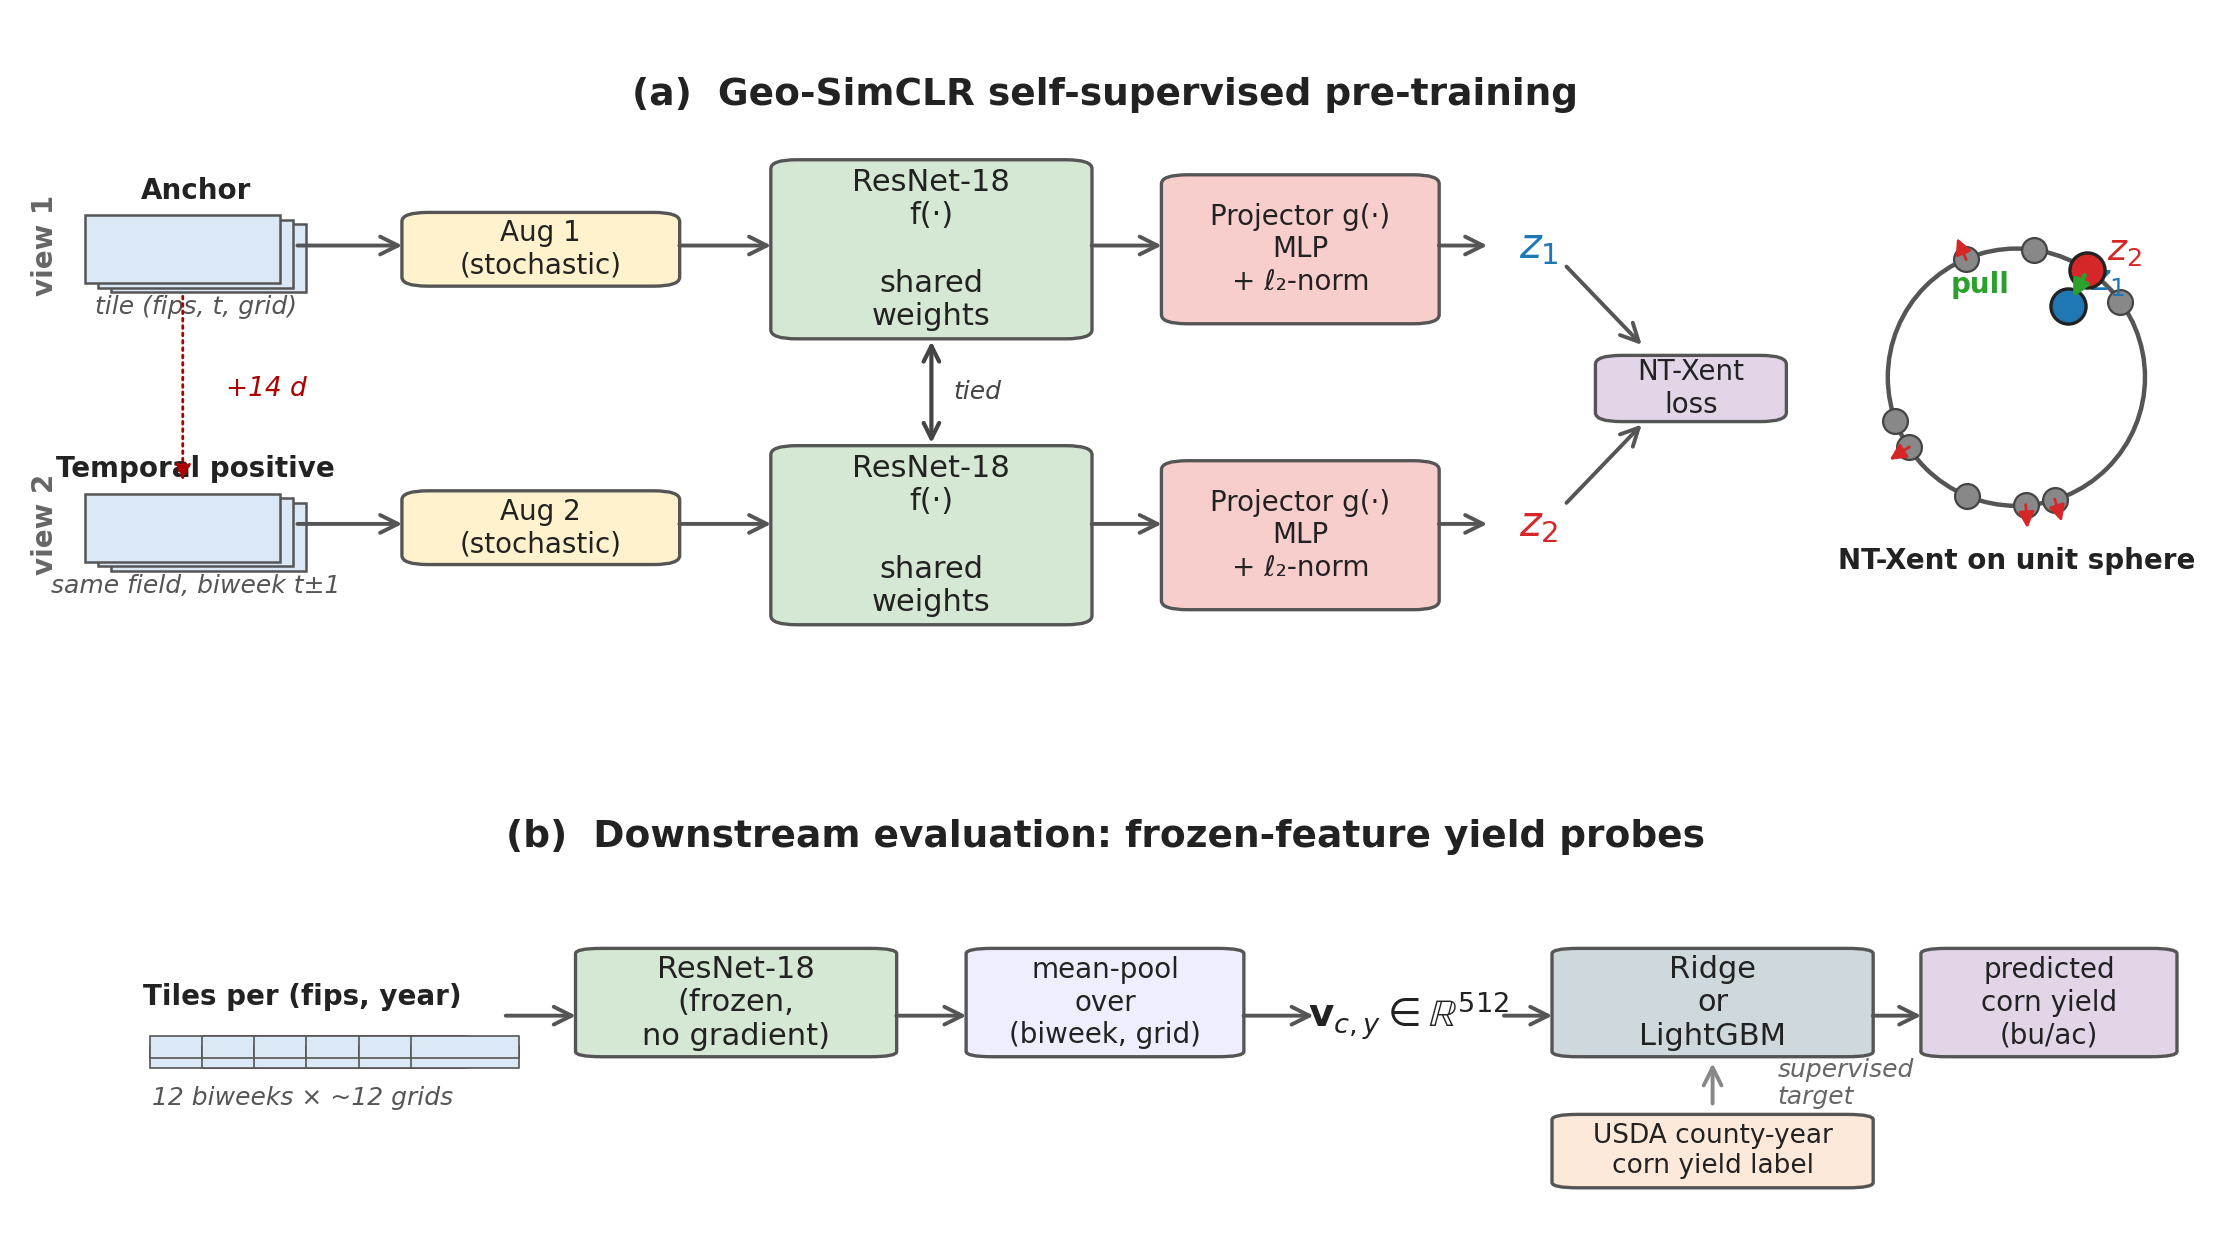
\includegraphics[width=\linewidth]{fig01_pipeline.png}
  \caption{Geo-SimCLR pipeline. (a) Self-supervised pre-training: an anchor tile
  and its same-field temporal positive (biweek $t \pm 1$, $\sim$14 days apart)
  are independently augmented, encoded by a shared ResNet-18 with a tied
  projection head, and the two $\ell_2$-normalised projections $z_1, z_2$ are
  pulled together while all other batch members act as negatives via NT-Xent.
  (b) Downstream evaluation: each county-year's tiles are passed through the
  frozen encoder, mean-pooled into a single 512-d county-year vector, and fed
  to a Ridge or LightGBM probe whose target is the USDA county-year corn yield.}
  \label{fig:pipeline}
\end{figure}

% --- Figure 2: real augmentation examples ---
\begin{figure}[H]
  \centering
  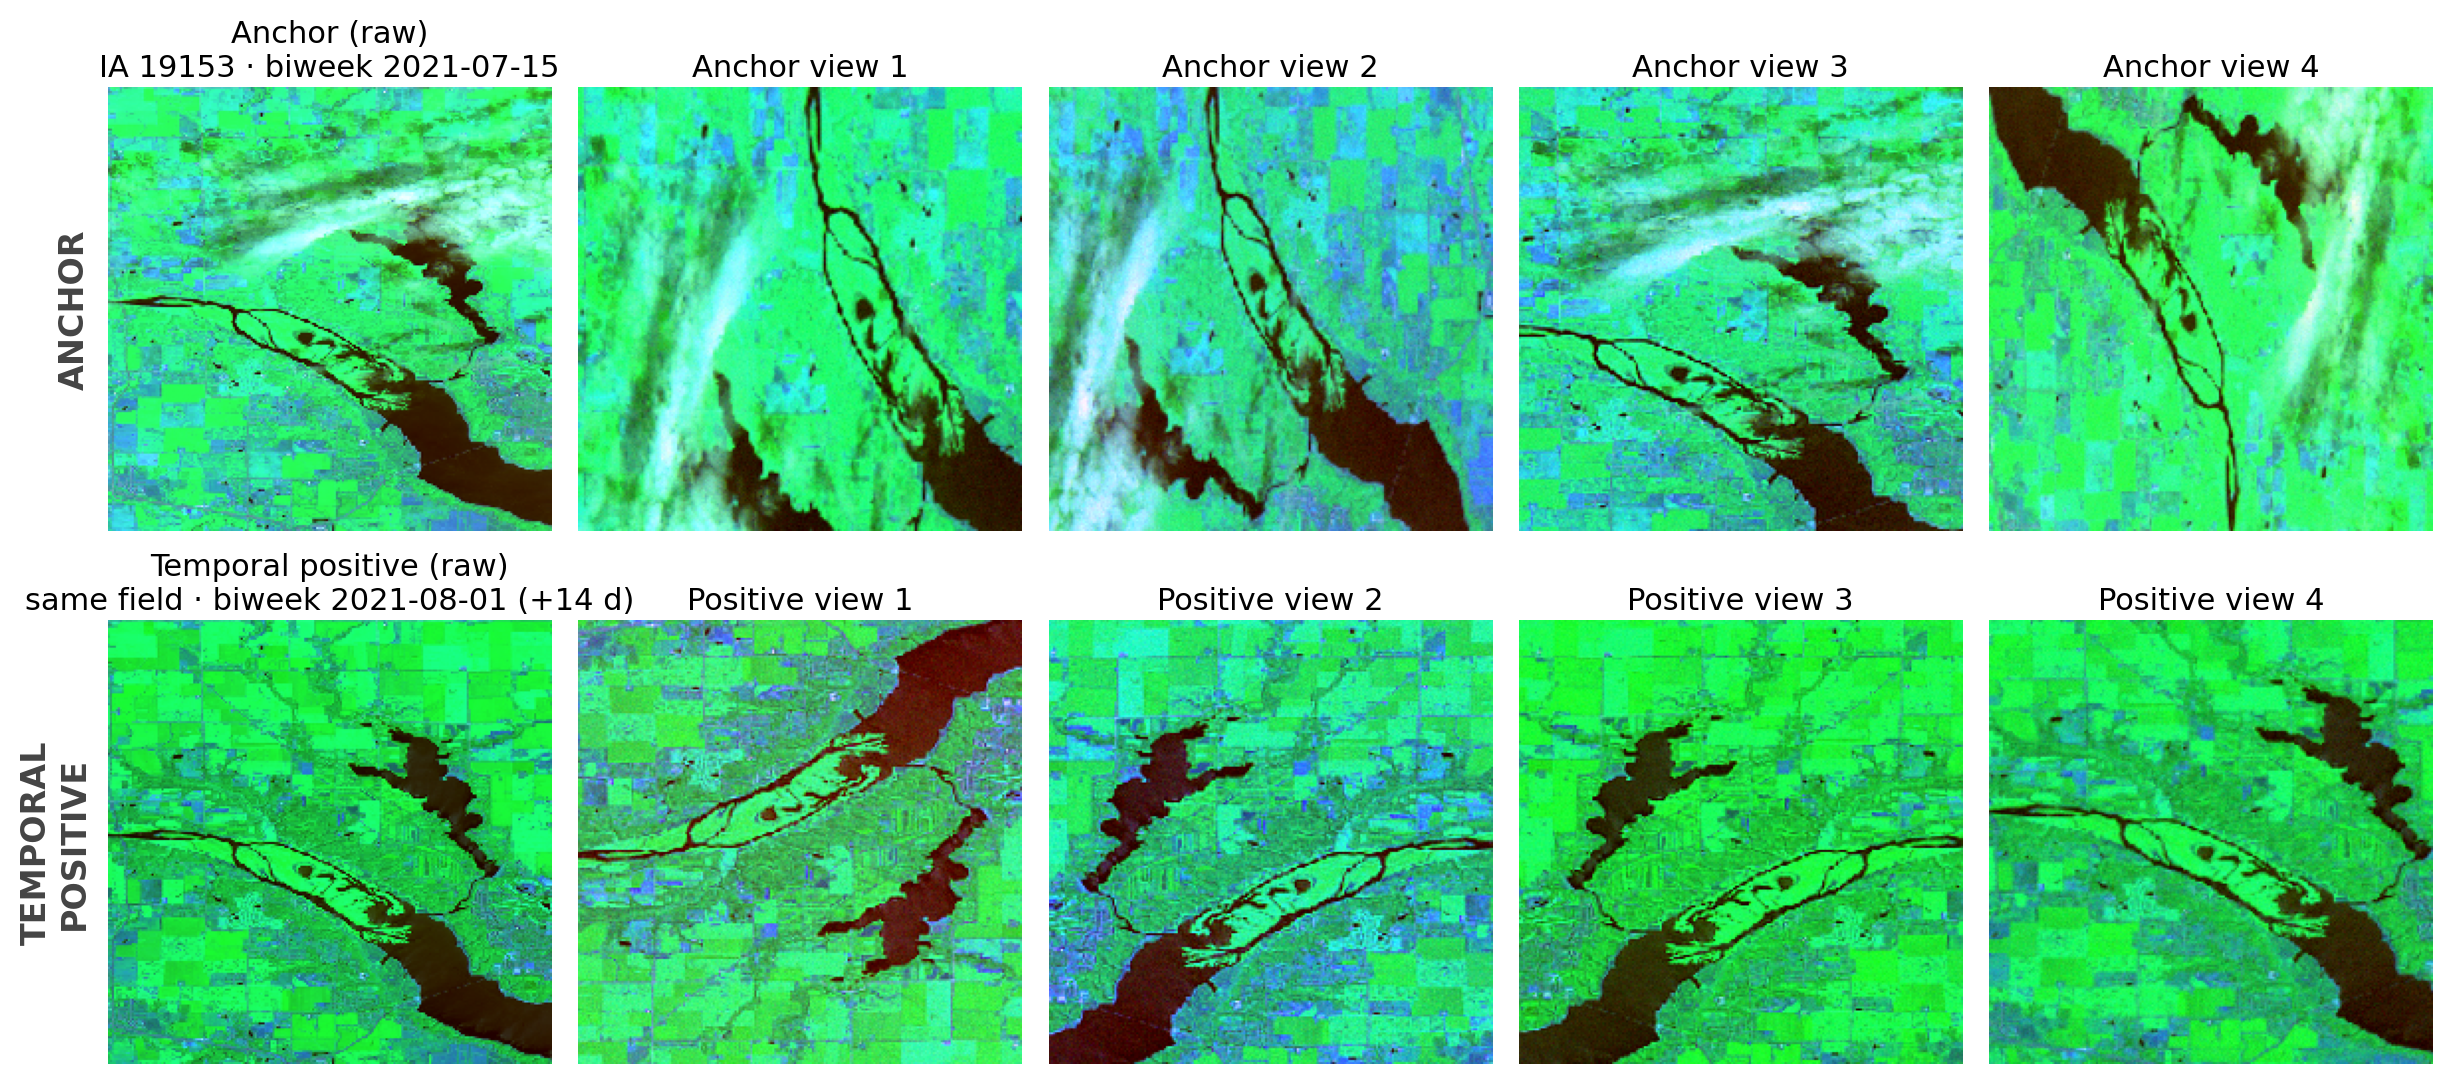
\includegraphics[width=\linewidth]{fig02_augmentation_examples.png}
  \caption{Geo-SimCLR pre-text task on real Sentinel-2 tiles, rendered in
  agriculture false-colour (SWIR1$\to$R, NIR$\to$G, Blue$\to$B). Top row: an
  anchor tile (Polk County, IA, 2021-07-15) and four independent stochastic
  draws of the augmentation pipeline. Bottom row: the temporal positive (same
  county and grid index, 2021-08-01, $+14$\,d) and four independent draws.
  The contrastive loss asks the encoder to make all eight augmented views
  similar to each other and dissimilar to other batch members. Augmentations
  are: random h/v flip, random rot90, random crop 160--208 px $\to$ resize 224,
  sharpness $\times 2.0$ with $p=0.5$, per-band intensity jitter
  $\times U[0.8,1.2]$ with $p=0.8$, per-band Gaussian noise $\sigma=0.02$, and
  per-band $z$-score. Spectral band dropout, RGB colour jitter, and mixup are
  deliberately omitted (incompatible with three-band EO + temporal-pair
  semantics).}
  \label{fig:aug-examples}
\end{figure}

\subsection{Data}
\label{sec:methods-data}
We use the CropNet release of Sentinel-2 imagery \citep{lin2024cropnet} for the
seven largest U.S.\ Corn Belt states (Iowa, Illinois, Indiana, Minnesota,
Nebraska, Ohio, South Dakota) over 2017--2022, restricted to the growing season
(April--September) at biweekly cadence. Each county is partitioned into
$\sim$12 grids of $9\times 9$\,km, each grid stored as a $224\times 224$\,px
tile at $\sim$40\,m/pixel resolution. We use the agriculture false-colour
band combination (B02 Blue, B08 NIR, B11 SWIR1) as a 3-channel input.
Total scope: 616 unique counties, 44{,}140 county-biweek index rows,
852{,}726 grid tiles, and 3{,}126 USDA county-year corn-yield labels (the
$\sim$12\,\% of cells with no published yield are small low-acreage counties
suppressed for privacy by USDA). Figure~\ref{fig:data-summary} (Appendix) lays
out the geographic and temporal coverage.

We additionally compute \emph{per-pixel} NDVI from the CropNet B04+B08
quantised reference channels and biweekly-mean NDVI at the county level, used
for the hand-crafted baselines in Section~\ref{sec:methods-baselines}.
Figure~\ref{fig:ndvi-phen} (Appendix) shows the resulting per-state phenology
curves and the global peak-NDVI-vs-yield relationship.

\subsection{Geo-SimCLR}
The pre-training pipeline is illustrated in Figure~\ref{fig:pipeline}(a) and an
example pretext task on real tiles is shown in Figure~\ref{fig:aug-examples}.

\paragraph{Temporal positive pairs.}
A SimCLR positive pair is conventionally two stochastic augmentations of the
\emph{same} image. We instead construct positives as
\((\mathrm{tile}_{c,t,g},\,\mathrm{tile}_{c,t \pm 1,g})\) -- the same county
$c$ and grid index $g$ at adjacent biweeks $t$ and $t\pm 1$. Both tiles are
then independently augmented before being fed through the shared encoder. This
forces the representation to be invariant to short-term weather, illumination,
and atmospheric noise (which differ across consecutive Sentinel-2 passes of
the same field) while remaining sensitive to slowly-varying canopy state.
After dropping anchors whose county lacks a CRD assignment in the lookup
($\sim 4.7\,\%$), we obtain 644{,}922 anchors per epoch.

\paragraph{CRD-balanced anchor sampling.}
Without intervention, batches drawn uniformly at random over all anchors are
dominated by counties from the data-rich, large states (IA, NE), which makes
within-batch negatives systematically less climate-diverse. We therefore use a
\texttt{WeightedRandomSampler} with weights inversely proportional to each
anchor's Crop Reporting District frequency
($\mathrm{crd\_id} = \mathrm{state\_ansi} \times 100 + \mathrm{asd\_code}$),
yielding 61 unique CRDs across the seven states. Each batch is therefore
agro-climatically diversified on average without explicit hard-negative mining.

\paragraph{Safe satellite-aware augmentations.}
Per view we apply, in order: random horizontal flip ($p=0.5$), random vertical
flip ($p=0.5$), random rot90 with $k\!\in\!\{1,2,3\}$ ($p=0.75$), random crop
to side length $\in [160, 208]$\,px followed by bilinear resize back to 224\,px,
random sharpness $\times 2.0$ ($p=0.5$), per-band intensity jitter $\times
U[0.8,1.2]$ ($p=0.8$), per-band Gaussian noise $\sigma=0.02$ in normalised
$[0,1]$ space, and per-band $z$-score normalisation. We deliberately omit
three augmentations that are standard in RGB SimCLR but inappropriate here:
spectral band dropout (too destructive on three channels), RGB-flavoured
colour jitter (we have no R/G/B channels in the conventional sense), and mixup
(would conflate distinct fields and break the temporal-pair semantics).

\paragraph{Architecture and loss.}
The encoder $f$ is a torchvision ResNet-18 trained from scratch (11.18\,M
backbone parameters, no input adapter -- the default 3-channel
$7\times 7$ \texttt{conv1} accepts our 3-band tiles directly). The projection
head $g$ is a 2-layer MLP $512 \to 256 \to 128$ with BatchNorm + ReLU; its
$\ell_2$-normalised 128-d output $z = g(f(x)) / \|g(f(x))\|_2$ feeds the
NT-Xent loss \citep{chen2020simclr},
\begin{equation}
\label{eq:ntxent}
\mathcal{L}_{i \to j} = -\log
  \frac{\exp(z_i^\top z_j / \tau)}{\sum_{k=1}^{2N} \mathbf{1}_{[k\neq i]} \exp(z_i^\top z_k / \tau)},
\end{equation}
with temperature $\tau = 0.2$ and $2N-1$ in-batch negatives ($N=1024$).
The total parameter count (encoder + projector) is 11.34\,M. Training runs
for 50 epochs at batch size 1024 across 2 GPUs with AdamW
(lr $10^{-3}$, weight decay $10^{-4}$), a 5-epoch linear warm-up followed by
cosine annealing, and AMP mixed precision; full hyperparameters are in
Table~\ref{tab:hyperparameters}.

\subsection{Frozen-feature probe protocol}
\label{sec:methods-probe}
For downstream evaluation we freeze the pre-trained backbone and aggregate
tile features to one vector per (\textit{fips}, \textit{year}) cell by
mean-pooling first across grids within each biweek and then across biweeks.
Two probes are reported: \textbf{Ridge} regression with $\alpha=1$, and \textbf{LightGBM} \citep{ke2017lightgbm} with 300 trees,
learning rate 0.05, num\_leaves 31, min\_child\_samples 5, with 20-round early
stopping on a 2021 validation set when applicable.

\paragraph{Split-aware feature choice.}
A 7-state one-hot indicator and a year scalar can be appended to the encoder
features before fitting the probe. We report headline numbers under the
per-encoder split-aware choice that wins empirically for \emph{every} encoder:
on the time split, Ridge \emph{without} state+year features (a year scalar
extrapolated outside the training range hurts the linear model and trees clamp
at the boundary leaf, so adding it backfires); on the county split, LightGBM
\emph{with} state+year features (year is in-distribution and the trees extract
state-year structure cleanly). Table~\ref{tab:full-grid} in the appendix
records all eight $\{$probe$\} \times \{\pm$state-year$\} \times \{$split$\}$
configurations for full transparency.

\paragraph{Bootstrap CIs.}
All test-set $R^2$ and RMSE values are reported with bootstrap 95\,\%
confidence intervals computed from $n=200$ paired resamples of the held-out
$(y_{\text{true}}, \widehat y)$ pairs, percentiles 2.5/97.5.

\subsection{Baselines}
\label{sec:methods-baselines}
We benchmark Geo-SimCLR against five baselines spanning the full chain from
hand-crafted indices to large foundation models.

\textbf{Hand-crafted NDVI} (six specifications, Table~\ref{tab:baselines}):
peak NDVI scalar; growing-season summary (6 features); biweekly NDVI series
(12 features); state+year one-hots; state+year + biweekly NDVI (the strongest
non-DL specification with 20 features); state+year + peak NDVI.
Models are Ridge or LightGBM per the table.

\textbf{Random ResNet-18.} Identical architecture to Geo-SimCLR but with a
freshly Kaiming-normal-initialised backbone, never trained. This serves as a
sanity baseline: mean-pooled random conv features after BatchNorm capture
colour and texture statistics correlated with vegetation.

\textbf{DINOv2-base} \citep{oquab2024dinov2}: 768-d frozen ViT pre-trained on
142\,M natural RGB images. We feed the AG bands as RGB slots
$(\text{R}, \text{G}, \text{B}) \leftarrow (\text{B02}, \text{B08}, \text{B11})$
and use the CLS token embedding. 85.7\,M parameters.

\textbf{Prithvi-EO 2.0} \citep{jakubik2023prithvi}: 1024-d frozen ViT
pre-trained on Harmonised Landsat-Sentinel imagery, expecting a 6-band HLS
input. Since CropNet only provides 3 of the 6 bands (B02, B08, B11), we
channel-pad the missing 3 with zeros at inference. 303.9\,M parameters.
This input mismatch is a documented limitation of the baseline rather than a
property of Prithvi itself: the model's effective rank on our channel-padded
inputs collapses to $\sim 1.7 / 1024$ in our diagnostics, severely
under-using its capacity.

\textbf{ConvLSTM} \citep{shi2015convlstm} as a supervised end-to-end imagery
comparator: a per-frame ResNet-18 (random init) producing 512-d per biweek,
followed by a single-layer LSTM (hidden 256) and an MLP head with dropout 0.2,
trained on $z$-scored yields with image augmentation applied identically to all
12 biweek frames. Total $\sim$12.4\,M parameters; full hyperparameters in
Table~\ref{tab:hyperparameters}.

\subsection{Splits}
\label{sec:methods-splits}
We report two complementary generalisation settings.
\textbf{Time split:} train 2017--2020 / val 2021 / test 2022. This is the
strict, no-look-ahead in-season-forecast benchmark: no 2022 tile -- not even
through positive pairs -- enters pre-training. 
\textbf{County split:} a random 20\,\% of FIPS codes is held out across all
six years. This is a spatial generalisation test: the model is asked to
predict yield in counties whose imagery was withheld from both pre-training
and probe fitting.

% =============================================================================
\section{Empirical results}
\label{sec:results}
% =============================================================================

\subsection{Headline encoder comparison}
\label{sec:results-headline}
\begin{table}[H]
\centering
\caption{Test-set $R^2$ and RMSE (bushels per acre) by encoder on 7-state US Corn Belt corn yield,
under the per-encoder split-aware probe choice. The time-split column uses Ridge with no state+year
features; the county-split column uses LightGBM with state+year features (the empirical winner of
both \{Ridge, LightGBM\} $\times$ \{with, without state+year\} grids for every encoder; see
Table~\ref{tab:full-grid}). Square brackets are bootstrap 95\% confidence intervals from $n\!=\!200$
paired resamples of held-out predictions; bold marks the column winner among the deep-learning rows.}
\label{tab:headline}
\begin{tabular}{lcccccc}
\toprule
& & \multicolumn{2}{c}{\textbf{Time split}} & \multicolumn{2}{c}{\textbf{County split}} \\
\cmidrule(lr){3-4}\cmidrule(lr){5-6}
\textbf{Encoder} & \textbf{Params (M)} & \textbf{$R^2$} [95\% CI] & \textbf{RMSE} & \textbf{$R^2$} [95\% CI] & \textbf{RMSE} \\
\midrule
\textbf{Geo-SimCLR*} & 11.2 & \textbf{+0.669 [+0.597, +0.714]} & \textbf{19.03} & \textbf{+0.660 [+0.591, +0.732]} & \textbf{16.60} \\
DINOv2-base & 85.7 & +0.661 [+0.594, +0.710] & 19.25 & +0.602 [+0.525, +0.671] & 17.95 \\
Prithvi-EO 2.0 & 303.9 & +0.550 [+0.504, +0.588] & 22.17 & +0.519 [+0.443, +0.581] & 19.74 \\
Random ResNet-18 & 11.2 & +0.558 [+0.506, +0.604] & 21.96 & +0.583 [+0.509, +0.650] & 18.37 \\
ConvLSTM (E2E) & 12.4 & +0.551 [+0.487, +0.620] & 21.95 & -- & -- \\
Best NDVI baseline$^{a}$ & -- & +0.429 & 24.78 & +0.651 & 18.15 \\
\bottomrule
\end{tabular}

\vspace{0.5em}
\footnotesize\raggedright
$^{*}$~Our model.\quad
$^{a}$~Best NDVI baseline = state one-hot + year + 12 biweekly NDVI features, LightGBM
(strongest of six tabular NDVI specifications; see Table~\ref{tab:baselines}).
ConvLSTM is reported only on the time split.
\end{table}


\begin{figure}[H]
  \centering
  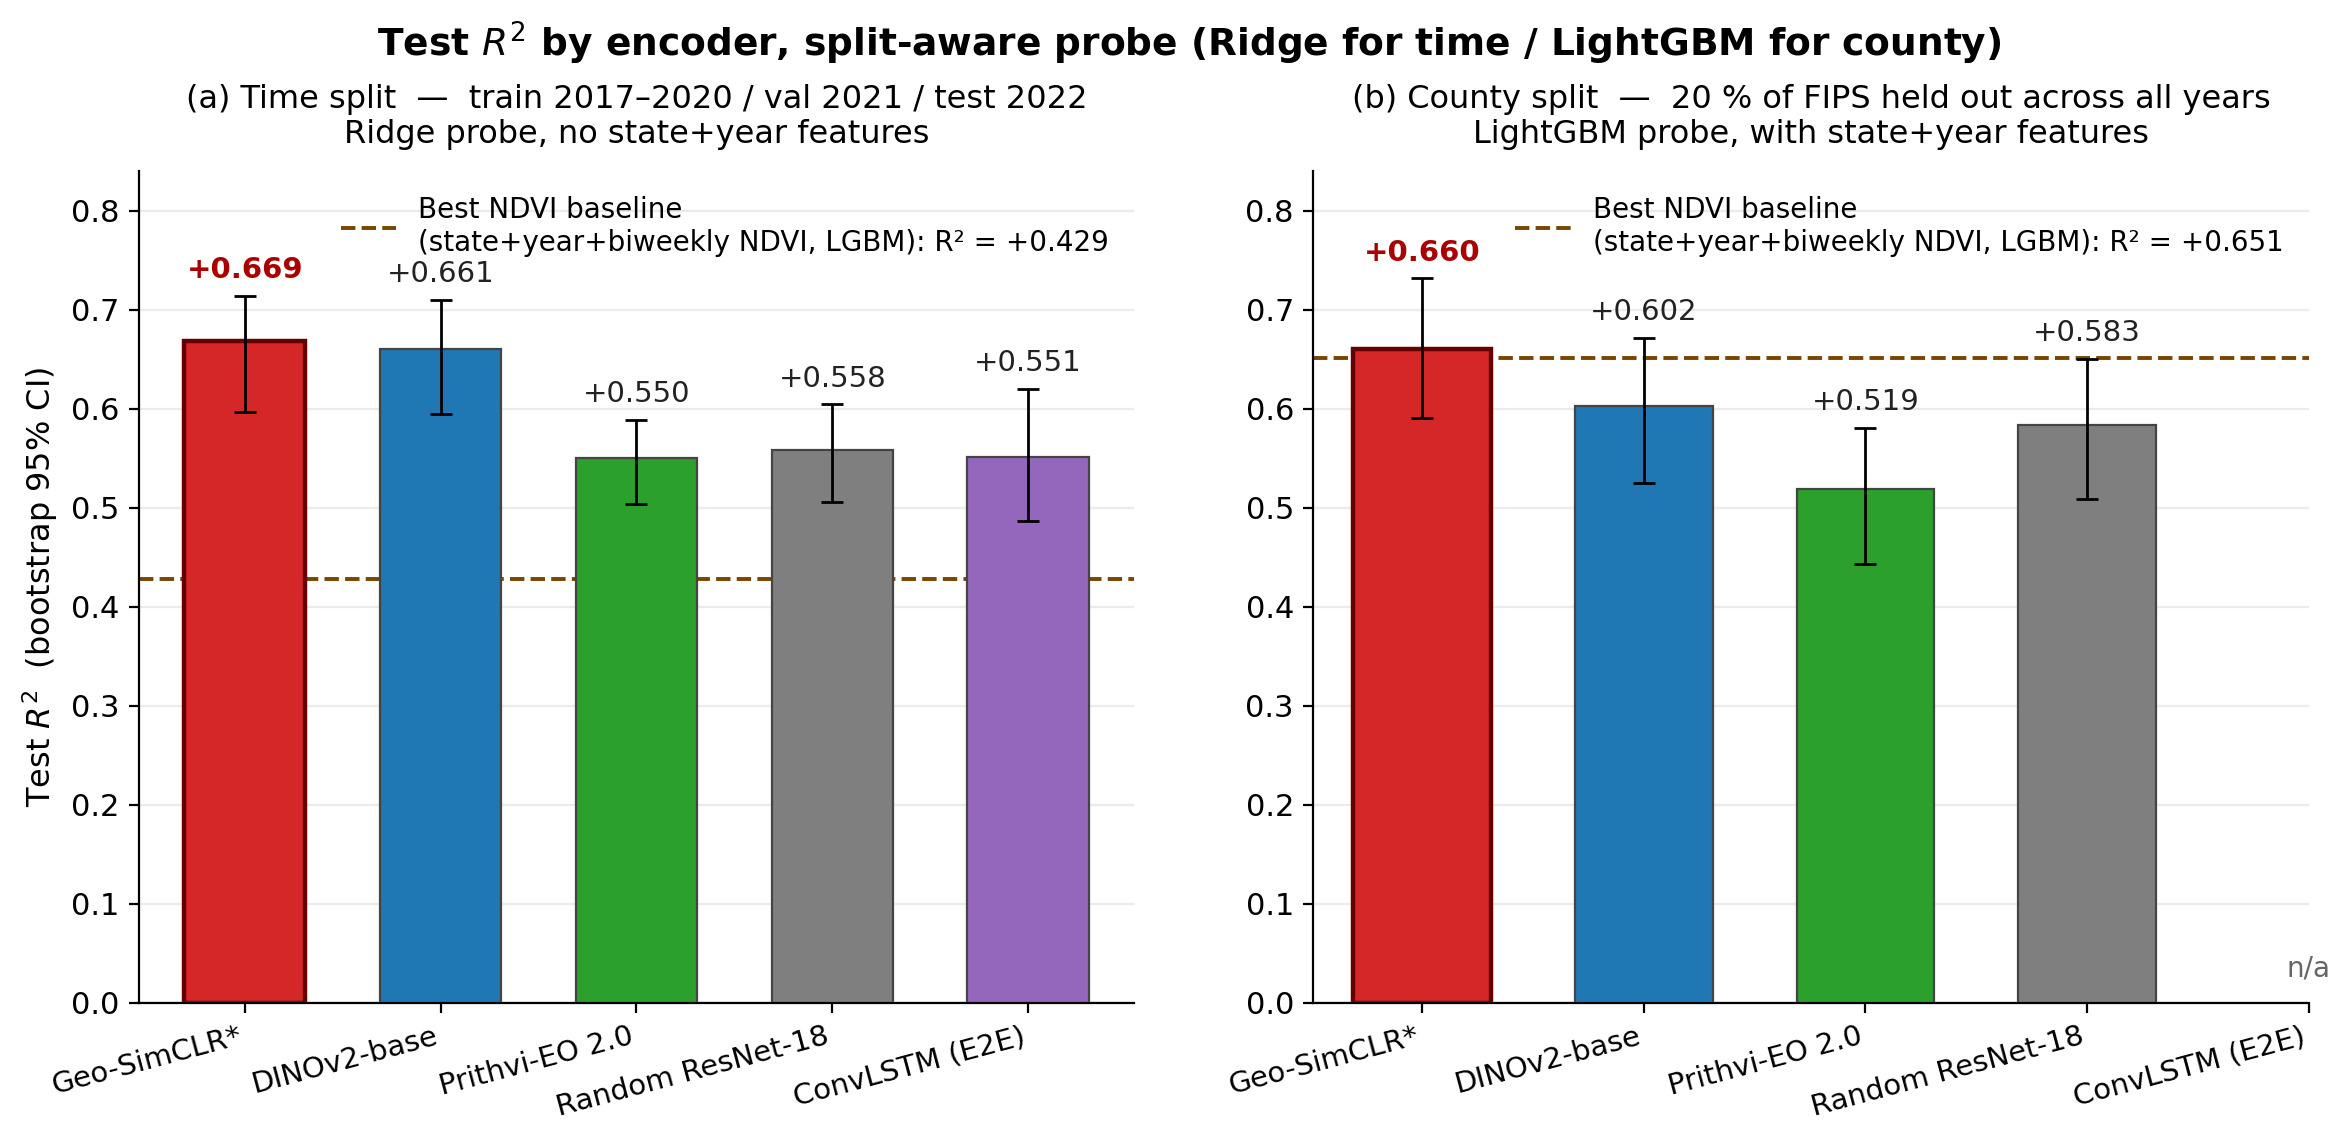
\includegraphics[width=0.98\linewidth]{fig05_encoder_comparison.png}
  \caption{Test $R^2$ by encoder under the per-encoder split-aware probe choice.
  Error bars are bootstrap 95\,\% CIs over $n\!=\!200$ paired resamples; the
  orange dashed line marks the strongest hand-crafted NDVI baseline
  (state + year + biweekly NDVI, LightGBM). \emph{Left:} time split; Ridge
  probe with no state+year features. \emph{Right:} county split; LightGBM probe
  with state+year features. ConvLSTM is run only on the time split.
  Geo-SimCLR is the per-panel winner on both splits.}
  \label{fig:encoder-comparison}
\end{figure}

Geo-SimCLR is the strongest single encoder on both splits
(Table~\ref{tab:headline}, Figure~\ref{fig:encoder-comparison}). On the time
split it reaches test $R^2 = 0.669$ \,[\,0.597, 0.714\,] with RMSE
$19.0$\,bu/ac, beating the strongest non-DL baseline by $+0.24\,R^2$ and the
supervised end-to-end ConvLSTM by $+0.118\,R^2$ -- a clean win in the
``frozen-features-and-linear-probe beats supervised end-to-end'' direction.
On the county split Geo-SimCLR reaches $R^2 = 0.660$ \,[\,0.591, 0.732\,] with
RMSE $16.6$\,bu/ac. Here the strongest tabular baseline (state+year +
biweekly NDVI LightGBM) is closer at $R^2 = 0.651$, because year and state are
in-distribution for the county split and absorb a large fraction of the
yield variance independently of imagery; the imagery-driven margin is therefore
narrow ($+0.009\,R^2$) but consistent across both Ridge and LightGBM probe
choices.

\paragraph{Probe-choice consistency.} The split-aware probe pattern is not
cherry-picked to favour one encoder. As Table~\ref{tab:full-grid} (appendix)
documents, Ridge beats LightGBM on the time split for every one of the four
DL encoders, and LightGBM with state+year features beats every alternative on
the county split for every encoder. DINOv2-base narrowly outranks Geo-SimCLR
on a handful of off-headline cells (most notably time-split / LightGBM /
$+$state-year, by $\sim$$+0.04\,R^2$); Geo-SimCLR wins or ties on the
empirically-best cell for every encoder.

\subsection{Hand-crafted NDVI baselines}
The six NDVI specifications (Table~\ref{tab:baselines}) reproduce well-known
patterns: the biweekly-NDVI series (12 features) substantially outperforms the
peak-NDVI scalar on both splits (e.g.\ $R^2$ $0.475$ vs.\ $0.261$ on the
county split), capturing the canopy phenology that a single August snapshot
misses; and adding state+year one-hots yields the strongest non-DL specification
on both splits ($R^2 = 0.429$ time, $0.651$ county). The county-split numbers
are systematically larger than the time-split numbers because year-to-year
variance (driven by weather and yield trend) exceeds across-county variance
for fixed years, and the time split asks the model to extrapolate to a year
it has never seen.

\begin{table}[H]
\centering
\caption{Hand-crafted NDVI baselines for 7-state corn-yield prediction (LightGBM and Ridge),
test-set $R^2$ and RMSE (bushels per acre) on both splits. Bold values are the per-column winner.}
\label{tab:baselines}
\begin{tabular}{lcccccc}
\toprule
& & & \multicolumn{2}{c}{\textbf{Time split}} & \multicolumn{2}{c}{\textbf{County split}} \\
\cmidrule(lr){4-5}\cmidrule(lr){6-7}
\textbf{Specification} & \textbf{\#feats} & \textbf{Model} & \textbf{$R^2$} & \textbf{RMSE} & \textbf{$R^2$} & \textbf{RMSE} \\
\midrule
Peak NDVI & 1 & Ridge & +0.141 & 30.38 & +0.261 & 26.43 \\
Growing-season summary & 6 & LightGBM & +0.200 & 29.33 & +0.363 & 24.54 \\
Biweekly NDVI series & 12 & LightGBM & +0.279 & 27.85 & +0.475 & 22.27 \\
State + year (no NDVI) & 8 & Ridge & +0.199 & 29.34 & +0.285 & 25.85 \\
\textbf{State + year + biweekly NDVI} & 20 & LightGBM & \textbf{+0.429} & \textbf{24.78} & \textbf{+0.651} & \textbf{18.15} \\
State + year + peak NDVI & 9 & Ridge & +0.235 & 28.68 & +0.427 & 23.26 \\
\bottomrule
\end{tabular}
\end{table}



\subsection{Why does the encoder ranking look like this?}
\label{sec:results-why}

The headline ranking in Table~\ref{tab:headline} -- Geo-SimCLR
$\succ$ DINOv2-base $\succ$ ConvLSTM \,$\sim$\, Random ResNet-18
$\succ$ Prithvi-EO 2.0 -- interpretation:

\textbf{Why Geo-SimCLR beats supervised end-to-end ConvLSTM.}
The SSL pretext task sees, conservatively, $\sim 6.4$ million
(anchor, positive, batch-of-1023-negatives) tuples per epoch over 50 epochs
on $\sim$852\,k unlabelled tiles, while ConvLSTM is trained on the
$\sim$2{,}100 supervised yield labels in its training fold. With this label
imbalance, learning the representation contrastively from unlabelled imagery
and then fitting a small probe is a higher-data-efficiency recipe than
back-propagating yield MSE through a deep CNN+LSTM end-to-end. The
$+0.118\,R^2$ margin on the time split is consistent with this view.

\textbf{Why Geo-SimCLR beats Prithvi-EO 2.0 despite Prithvi being EO-specialised
and 27$\times$ larger.}
Prithvi expects 6-band HLS input
(Blue, Green, Red, Narrow-NIR, SWIR1, SWIR2); we have 3-band CropNet AG
(Blue, NIR, SWIR1) and pad the missing three channels with zeros. This
channel-padding hits Prithvi unusually hard: its effective rank on our
padded inputs collapses to $\sim 1.7 / 1024$, leaving most of its capacity
unused. This is a documented baseline limitation, not evidence Prithvi is a
weak model in its trained regime; a fair comparison would require either
(i) a CropNet release with the full HLS band set or (ii) re-pre-training
Prithvi from scratch on 3-band inputs.

\textbf{Why DINOv2 nearly matches Geo-SimCLR (within $\sim$$0.06\,R^2$ at
$7.6\times$ more parameters).}
DINOv2 was trained on 142\,M natural RGB images with strong augmentations and
a self-distillation objective optimised for transfer; mean-pooling its CLS
token across many tiles is a robust feature even when the input is satellite
agriculture false-colour fed through RGB slots. This is consistent with recent
findings that large general-purpose SSL transfers surprisingly well to
satellite RGB-like inputs at no fine-tuning cost. Geo-SimCLR still wins on the
empirical headline because (i) the temporal-positive pretext task is
domain-aware and (ii) we evaluate at a fixed-modality budget where DINOv2's
natural-image biases occasionally hurt.

\textbf{Why Random ResNet-18 produces $R^2 > 0$.}
Mean-pooled random convolutional features after BatchNorm capture colour and
texture statistics that correlate with vegetation. The \emph{clean}
SSL gain is therefore not Geo-SimCLR's headline number but the gap to the
random baseline: $+0.111\,R^2$ on the time split and $+0.077\,R^2$ on the
county split.

\subsection{Self-supervised training trajectory}
\label{sec:results-trajectory}

\begin{figure}[H]
  \centering
  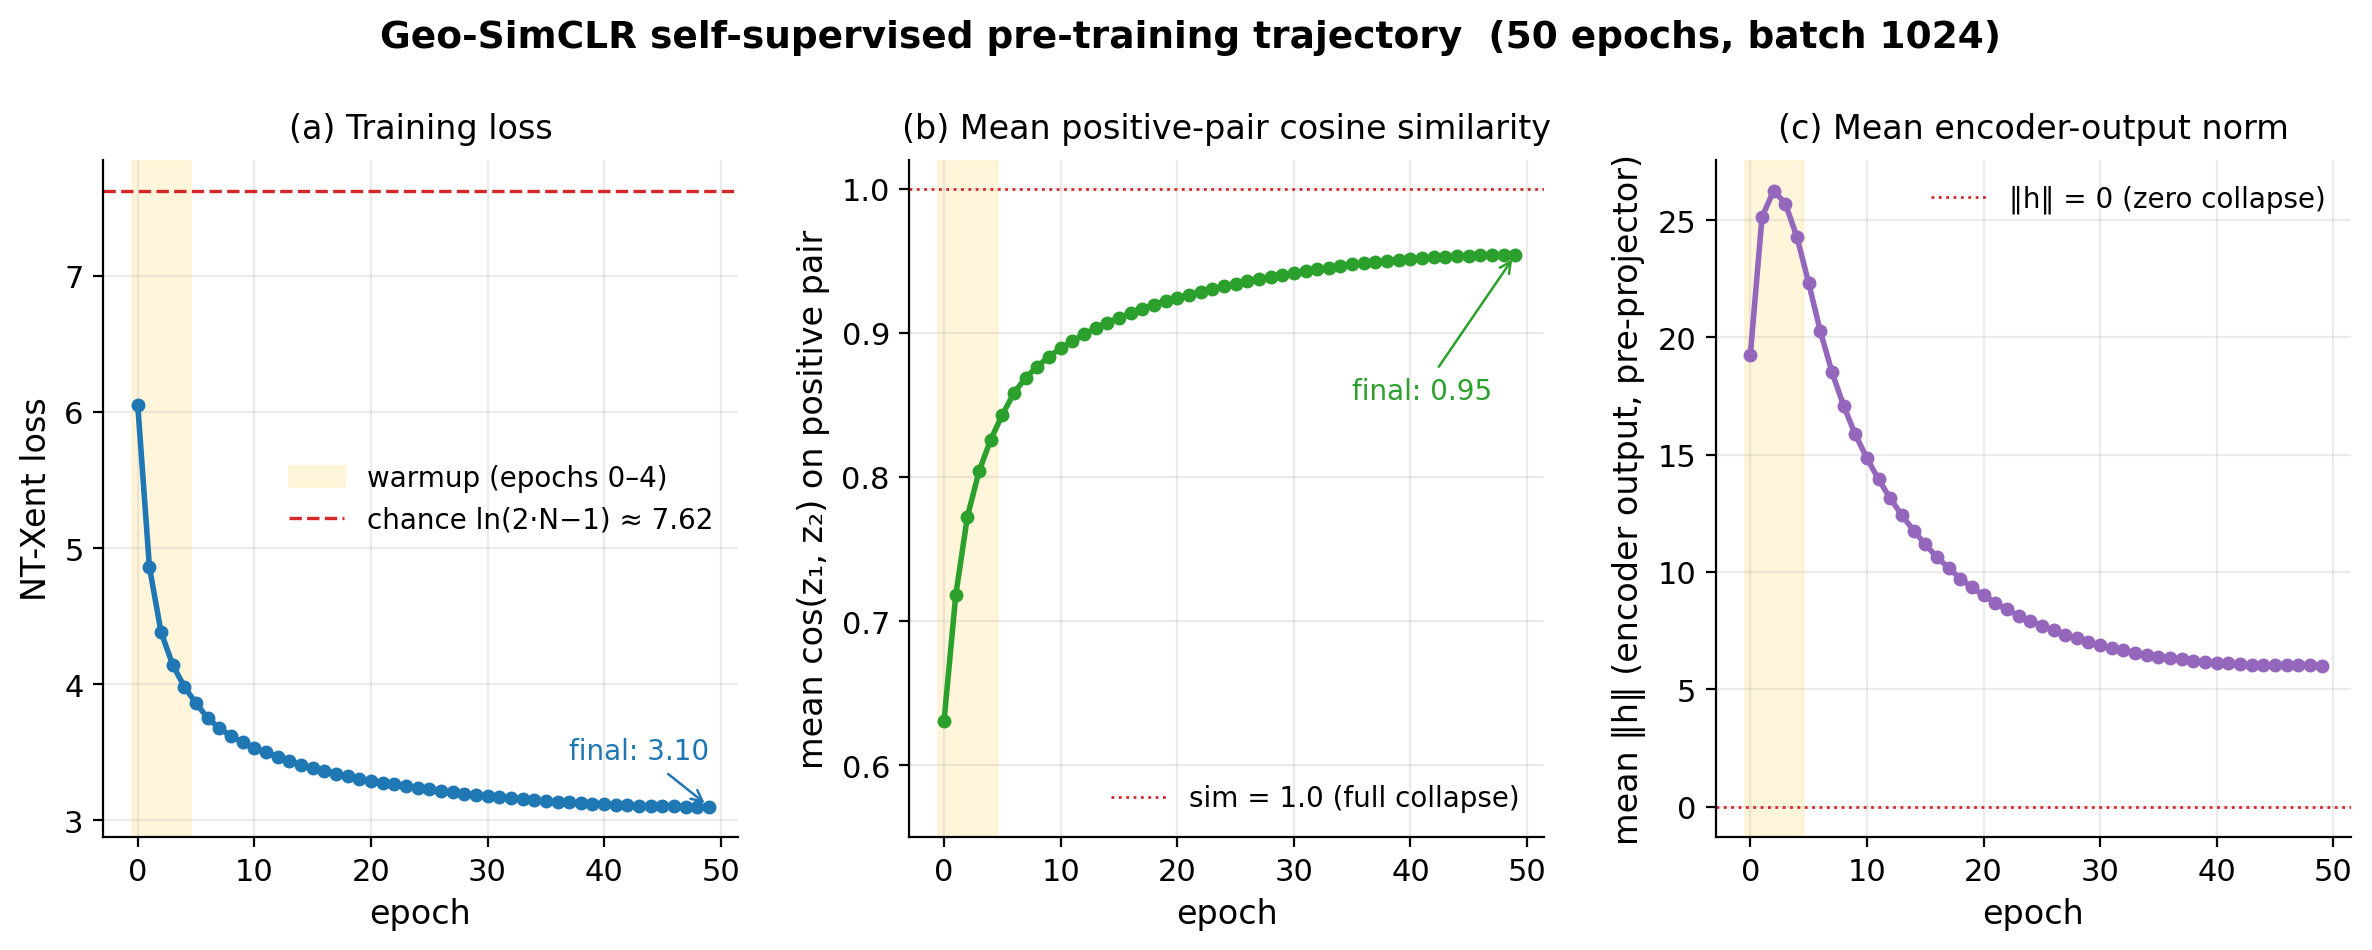
\includegraphics[width=\linewidth]{fig06_training_curves.png}
  \caption{Geo-SimCLR pre-training trajectory over 50 epochs at batch 1024.
  (a) NT-Xent loss falls cleanly from 6.05 at epoch 0 (already below the
  chance level $\ln(2N\!-\!1) \approx 7.62$) to 3.10 at epoch 49. (b) Mean
  positive-pair cosine similarity rises monotonically to $\sim$$0.95$ -- a
  warning that adjacent-biweek temporal positives are inherently easy
  (Section~\ref{sec:results-collapse}). (c) Mean encoder-output norm $\|h\|$
  is stable, ruling out the standard zero-collapse failure mode in which the
  encoder maps everything to the origin. The shaded yellow band marks the
  5-epoch linear LR warm-up.}
  \label{fig:training-curves}
\end{figure}

The training trajectory in Figure~\ref{fig:training-curves} shows clean,
non-pathological optimisation: loss converges from chance, and the encoder
output norm remains bounded. The one early warning sign is the monotone climb
of the mean positive-pair cosine similarity to $\sim$$0.95$. A
healthy SimCLR training trajectory tends to plateau much lower (typically
$0.5$--$0.8$ on natural images). However, the similarity starts at aroun $0.6$, so the proximity to 1 somewhat less surprising, but it does suggest the temporal-positive pretext task is too easy: the encoder can satisfy NT-Xent
by simply collapsing same-county-and-near-time pairs onto each other rather
than learning richer fine-grained features. We diagnose this collapse
quantitatively next.

\subsection{What did the encoder learn?}
\label{sec:results-mphate}

\begin{figure}[H]
  \centering
  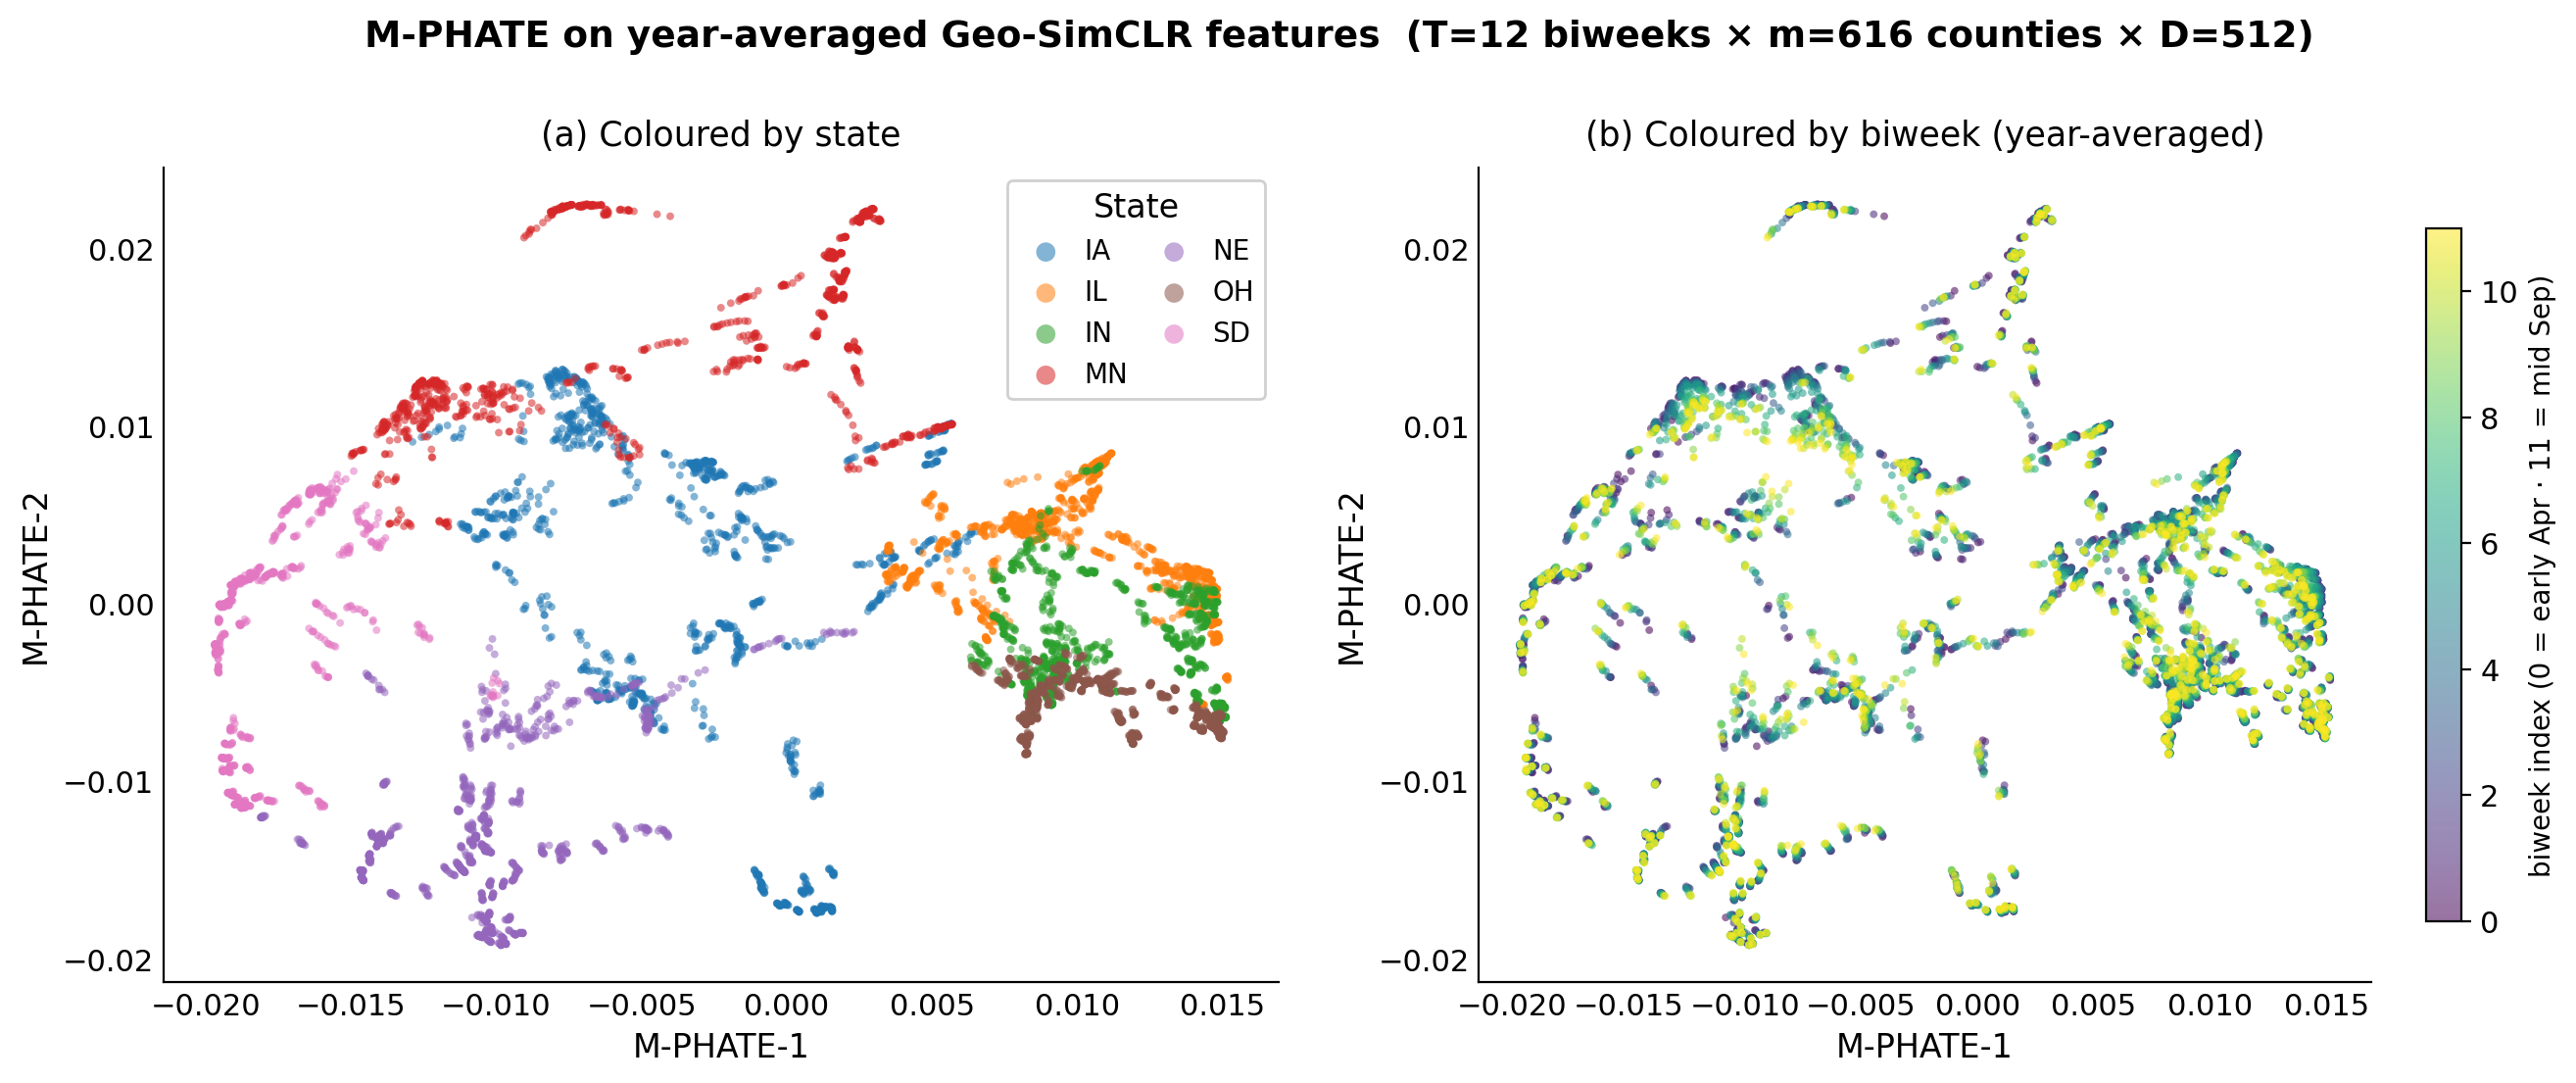
\includegraphics[width=\linewidth]{fig07_mphate.png}
  \caption{M-PHATE \citep{gigante2019mphate} 2-D embedding of Geo-SimCLR
  features on the year-averaged tensor (12 biweeks $\times$ 616 counties
  $\times$ 512 features), with intra-slice $k=5$ and inter-slice $k=6$
  neighbour kernels. (a) Coloured by state: state-coherent clusters separate
  cleanly. (b) Coloured by biweek index: biweek transitions are smooth but
  tightly overlapping within each state cluster, indicating that seasonal
  phenology is only weakly encoded relative to geographic identity. M-PHATE's
  inter-slice kernel imposes some temporal coherence by construction, so this
  is a generous upper bound on what the encoder learned about phenology.}
  \label{fig:mphate}
\end{figure}

The M-PHATE embedding (Figure~\ref{fig:mphate}) has two complementary
readings. State coloring -- the (a) panel -- produces clean,
geographically-coherent clusters: counties within the same state map to a
common region of the embedding, and adjacent states (IL/IN) cluster more
tightly with each other than with distant states (SD/MN). This is the
\emph{positive} side of the story: the encoder reliably encodes the
agro-climatic identity of each county. Biweek coloring -- the (b) panel --
shows the reverse pattern: biweeks blend smoothly within each state cluster
rather than tracing distinct phenological trajectories. M-PHATE's inter-slice
kernel imposes some temporal coherence by construction, so this is a generous
upper bound; the next subsection quantifies how much phenology actually
survives.

\subsection{Potential collapse diagnostic}
\label{sec:results-collapse}

\begin{figure}[H]
  \centering
  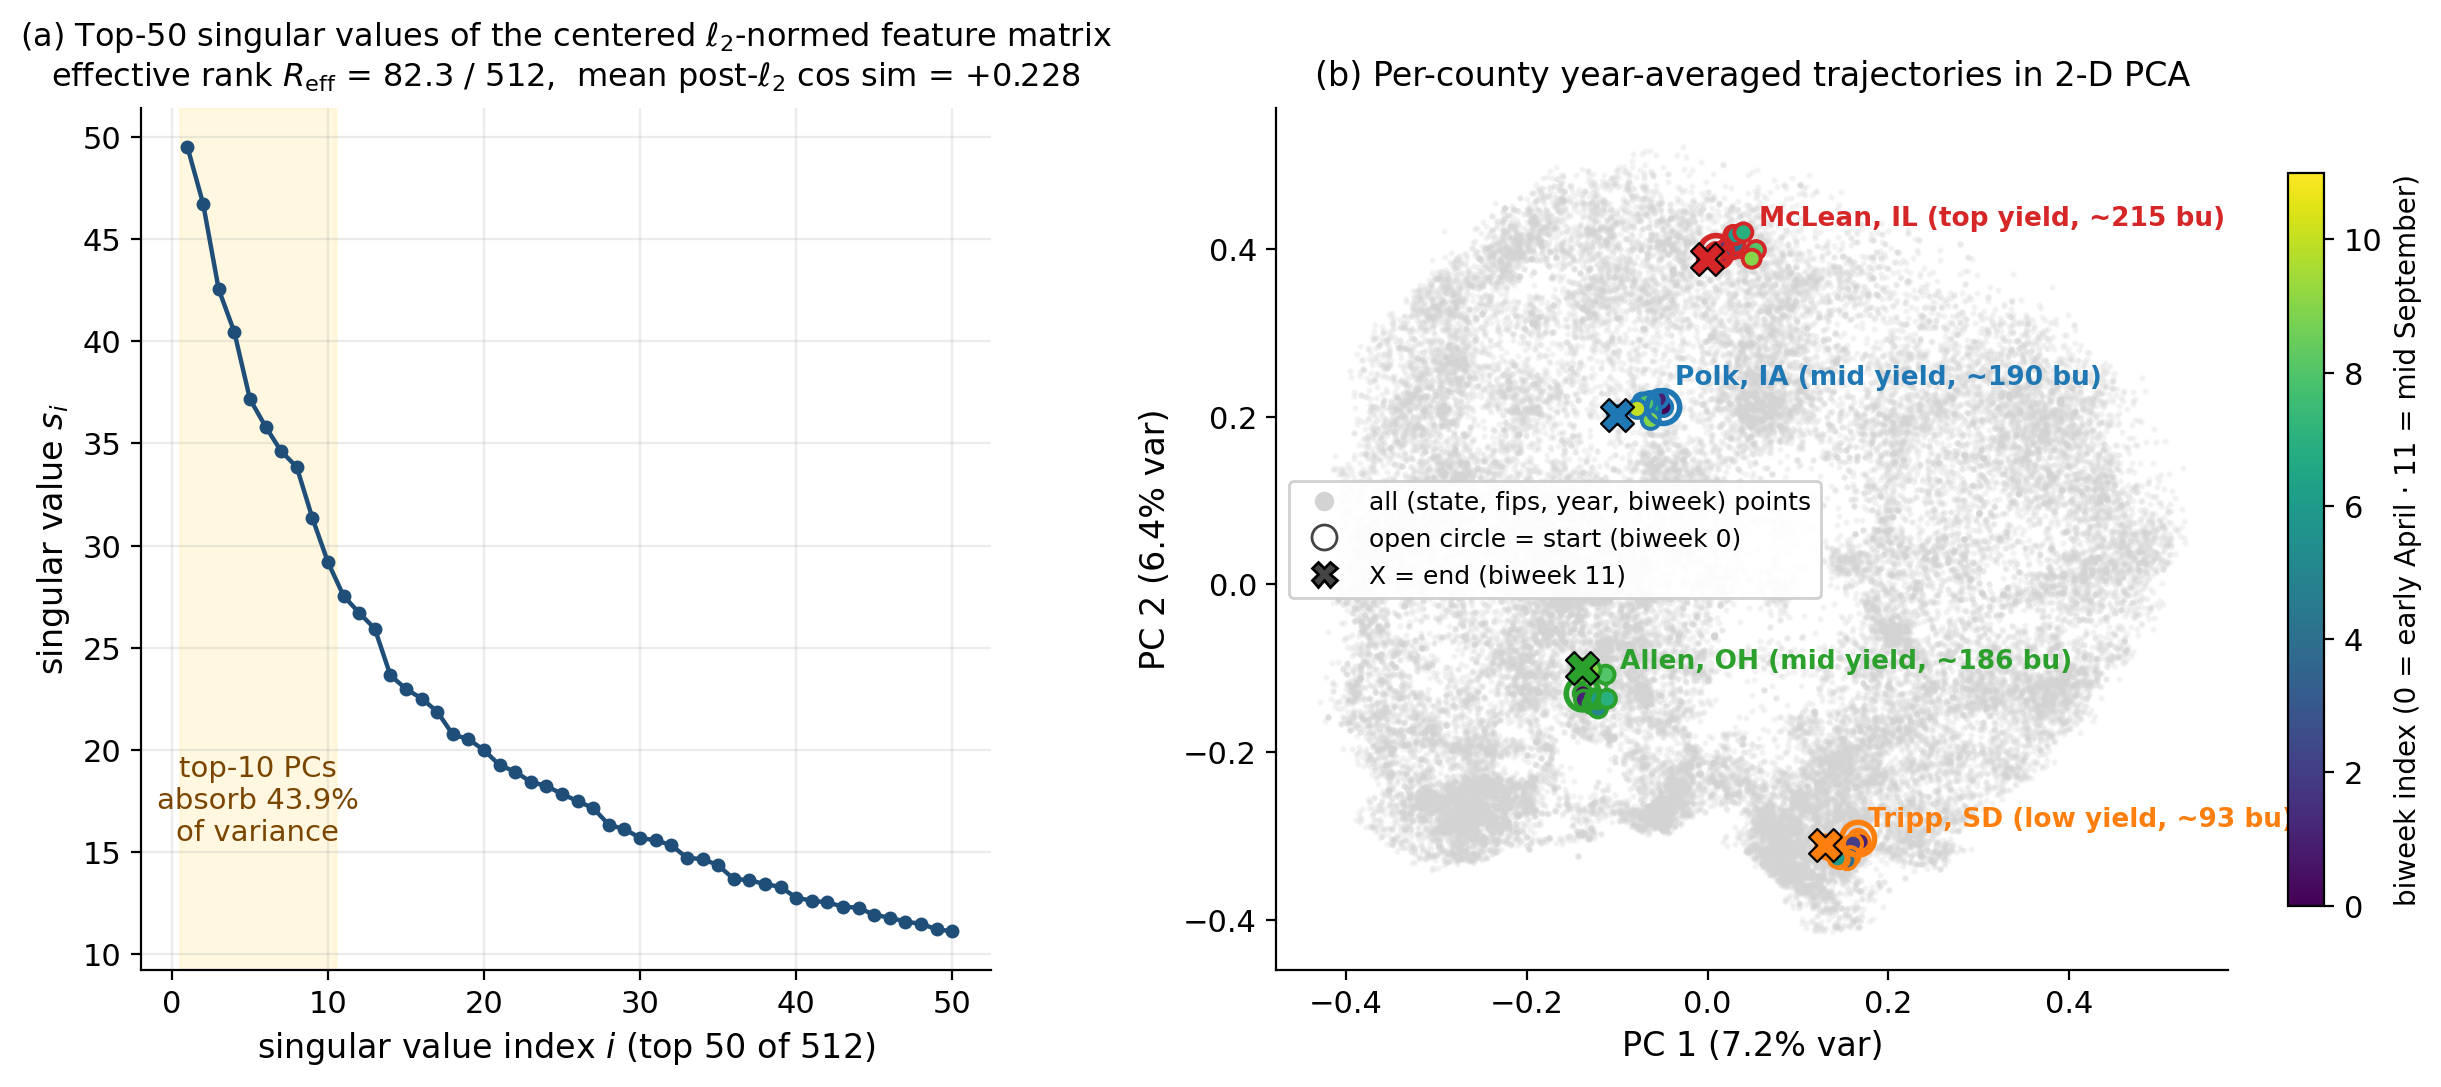
\includegraphics[width=\linewidth]{fig08_collapse.png}
  \caption{Dimensional-collapse diagnostic on the full $\ell_2$-normalised
  pooled feature matrix. (a) Top-50 singular values of the centered feature
  matrix; the shaded region marks the top-10 PCs, which already absorb 43.9\,\%
  of the variance, and the effective rank
  \(R_{\mathrm{eff}} = \exp(-\sum_i p_i \log p_i)\) of
  \citet{roy2007effrank} is 82.3 out of 512. (b) Per-county year-averaged
  trajectories in 2-D PCA for four hand-picked counties spanning the yield
  range; each county's 12 biweek points span only 4--6\,\% of the global
  pairwise distance, so the seasonal trajectory is compressed almost to a
  single point relative to the across-county spread.}
  \label{fig:collapse}
\end{figure}

\begin{table}[H]
\centering
\caption{Geo-SimCLR representation diagnostics on the full 7-state pooled feature matrix
($n\!=\!44{,}140$ tile vectors $\times\,512$ dimensions, $\ell_2$-normalized to match the cosine NT-Xent geometry).
Effective rank follows Roy and Vetterli (2007); cosine-similarity statistics are computed over
$n\!=\!2{,}000$ random tile-vector pairs.}
\label{tab:effrank}
\begin{tabular}{lc}
\toprule
\textbf{Diagnostic} & \textbf{Value} \\
\midrule
Number of pooled tile vectors & 44,140 \\
Embedding dimensionality $D$ & 512 \\
Effective rank $R_\mathrm{eff} = \exp(-\sum_i p_i \log p_i)$ & 82.3 \,/\, 512 \\
Top-1 PC variance fraction & 7.21\% \\
Top-10 PC variance fraction & 43.92\% \\
Top-30 PC variance fraction & 69.14\% \\
Singular-value ratio $s_0/s_1$ & 1.06 \\
Singular-value ratio $s_0/s_{10}$ & 1.80 \\
Within-county feature variance & 2.21e-04 \\
Between-county feature variance & 1.29e-03 \\
Variance ratio (within $/$ between) & 0.171 \\
Mean post-$\ell_2$ cosine similarity (random pairs) & +0.228 $\pm$ 0.137 \\
\bottomrule
\end{tabular}
\end{table}


The SVD spectrum and per-county PCA trajectories in Figure~\ref{fig:collapse}
provide quantitative confirmation of the qualitative M-PHATE finding. Three
numbers tell the story (Table~\ref{tab:effrank}). First, the effective rank of
the pooled, $\ell_2$-normalised feature matrix is $82.3 / 512$: the encoder
concentrates the data on a low-dimensional subspace using $\sim$16\,\% of its
nominal capacity. Second, the mean cosine similarity between random pairs of
$\ell_2$-normalised tile vectors is $+0.228$, far above the $\approx 0$
expected from a healthy SimCLR encoder
\citep{chen2020simclr,jing2022dimcollapse}. Third, the within-county feature
variance is only 17\,\% of the between-county feature variance: most of the
information in the embedding is which county the tile is from, not when in the
season it was taken or how that field is doing.

The PCA trajectories in Figure~\ref{fig:collapse}(b) make this concrete: each
county's 12 biweek points (early-April open circle through mid-September X
marker) span only 4--6\,\% of the global pairwise distance. A county imaged in
April and the same county imaged in September map to almost the same point in
the encoder's representation. This is the canonical signature of dimensional
collapse onto a single dominant direction (here: county identity). The
appendix figure (Figure~\ref{fig:phate-umap}) corroborates the same finding
through plain PHATE and UMAP, both of which produce ball-shaped embeddings
with significant state and biweek mixing.

We hypothesise the proximate cause is the same one Figure~\ref{fig:training-curves}(b)
flagged: same-county tiles separated by only $\pm 14$ days at $9$\,km
field scale are intrinsically very similar, and the contrastive objective can
satisfy NT-Xent by reinforcing static county identity rather than learning
fine-grained phenology. Section~\ref{sec:discussion} discusses concrete fixes.

\subsection{Pixel attribution via GradCAM}
\label{sec:results-gradcam}

\begin{figure}[H]
  \centering
  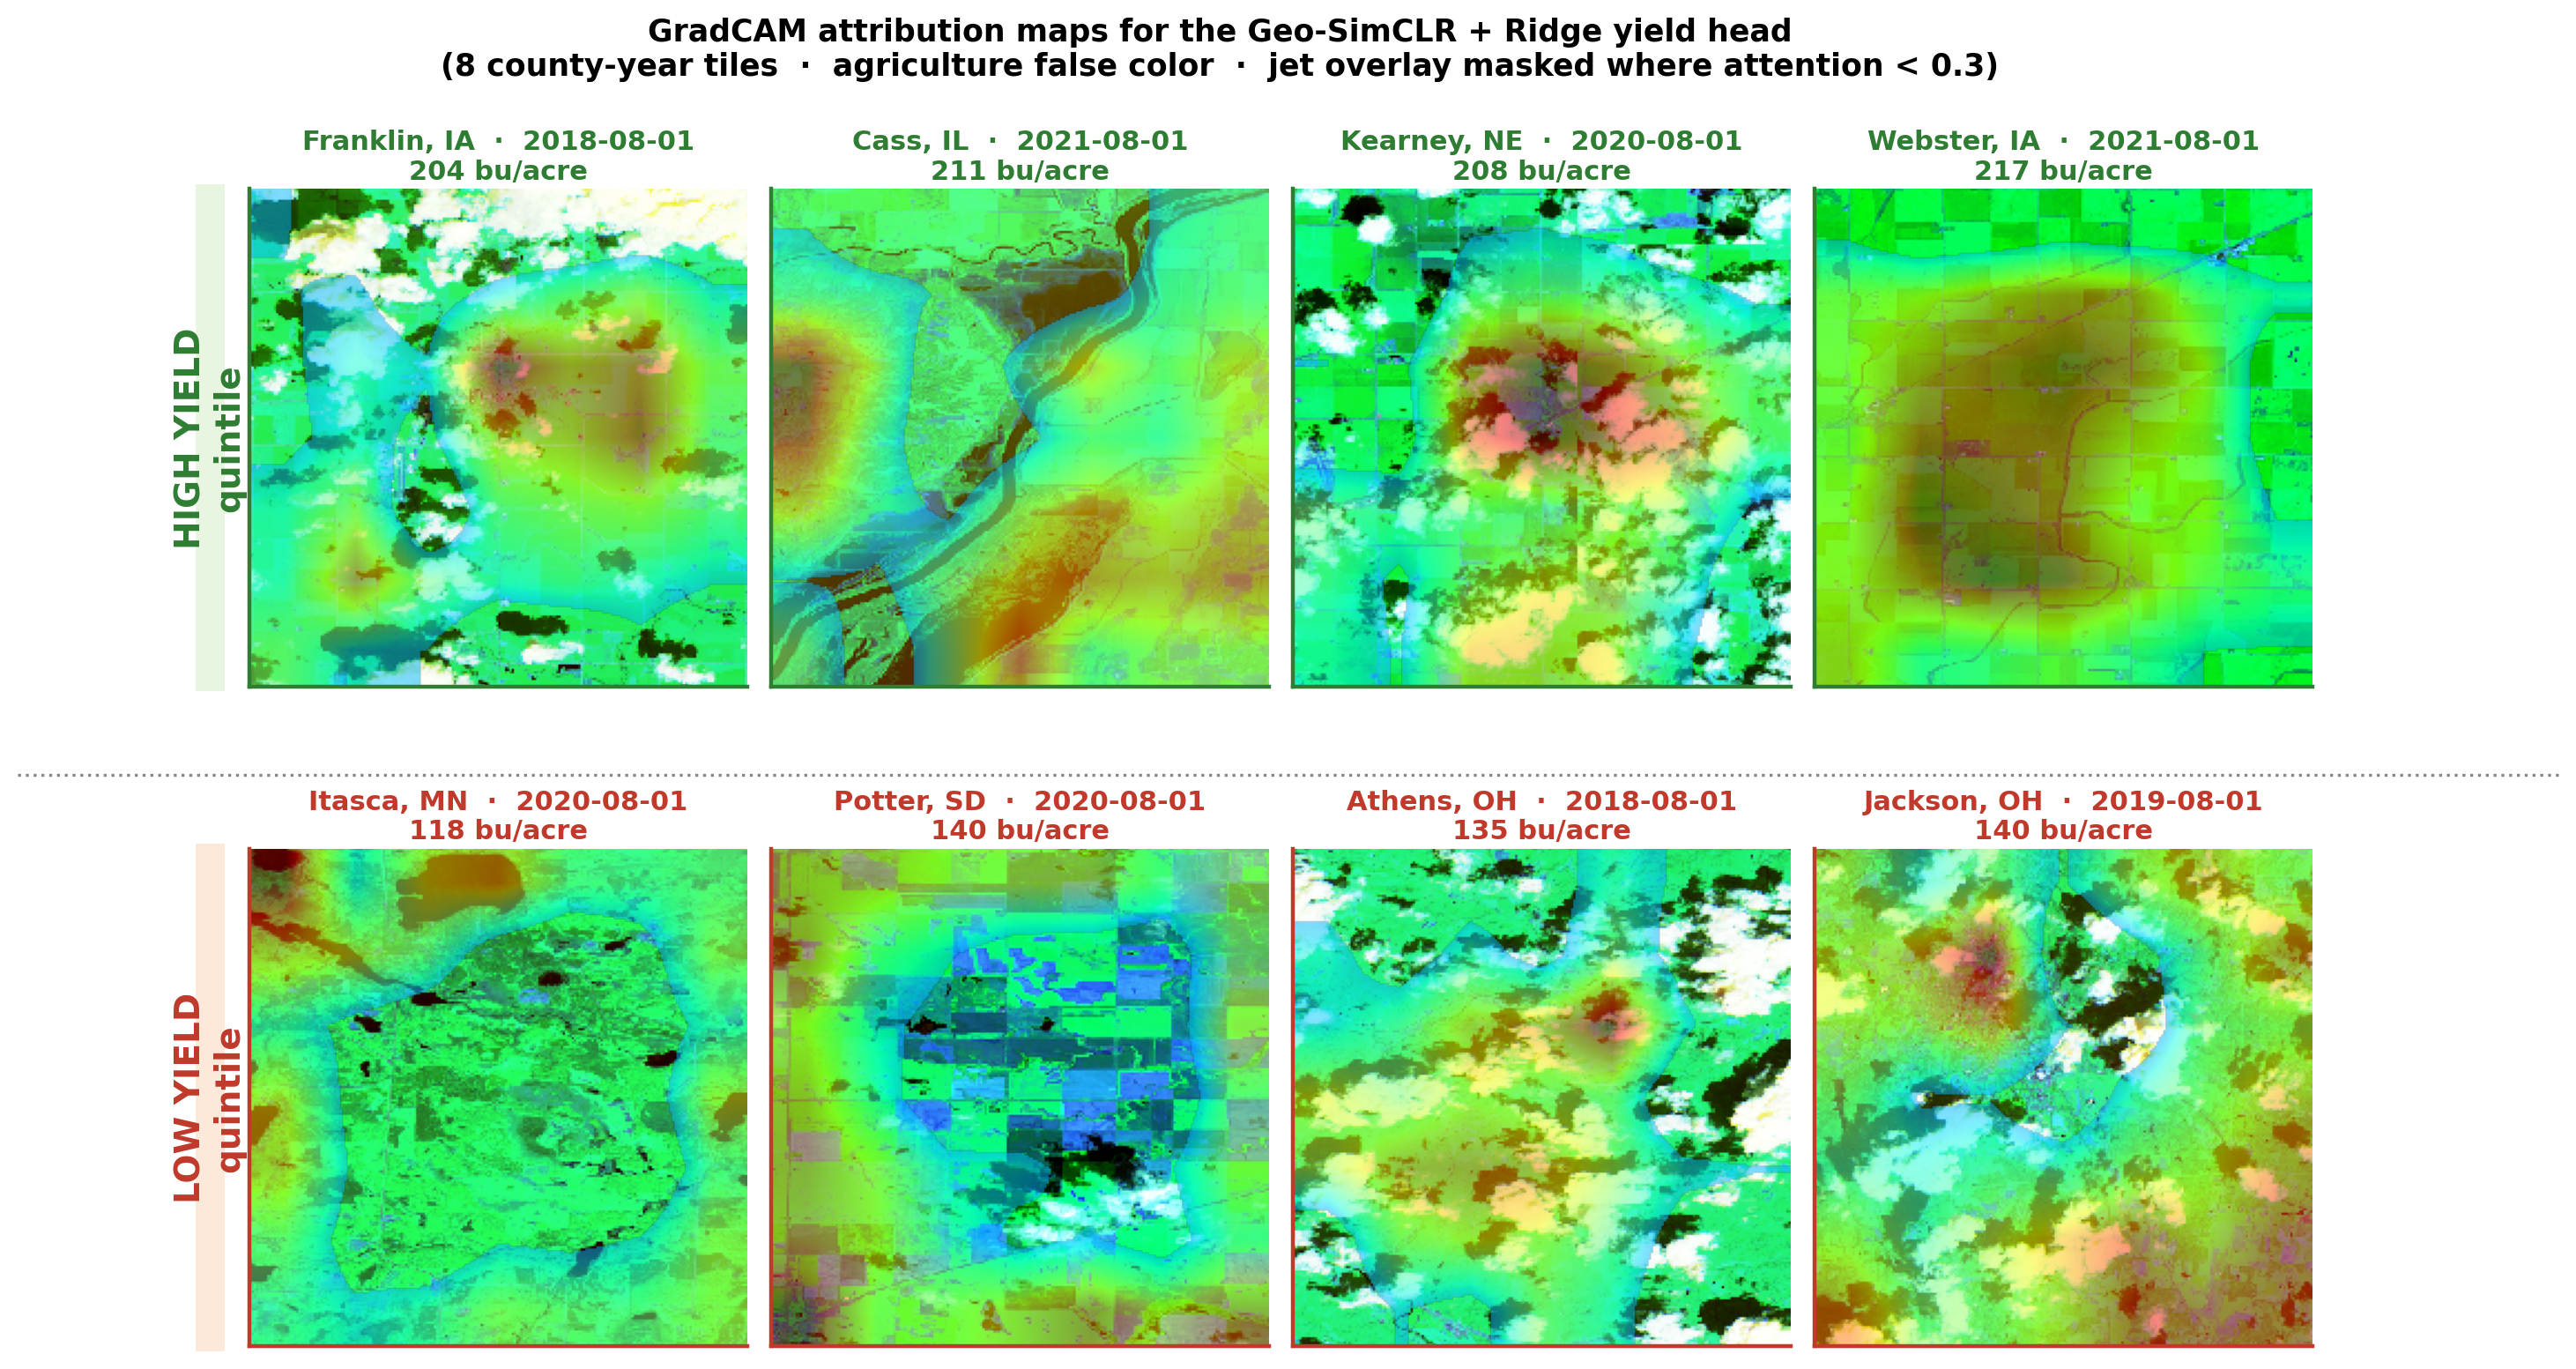
\includegraphics[width=\linewidth]{fig09_gradcam.png}
  \caption{GradCAM \citep{selvaraju2017gradcam} attribution maps for the
  composition of the frozen Geo-SimCLR encoder and a Ridge yield head, computed
  via Captum's \texttt{LayerGradCam} \citep{kokhlikyan2020captum} on
  \texttt{layer4[-1]}. Top row: four highest-yield-quintile county-years; bottom
  row: four lowest. Tiles are rendered in agriculture false-colour with a global
  2nd--98th-percentile contrast stretch; the jet overlay is masked to the top
  70\,\% of attention so only high-attention regions are coloured.}
  \label{fig:gradcam}
\end{figure}

The GradCAM maps in Figure~\ref{fig:gradcam} show the regions of each tile
that drive the encoder's contribution to the Ridge yield head. The pattern is
consistent across both yield extremes: attention concentrates on cropland
regions (the vivid green areas in agriculture false-colour) and de-emphasises
water bodies, urban pixels, and partially cloudy regions. Given the potential collapse, these maps should be interpreted as
\emph{cropland-vs-non-cropland attribution} -- the encoder tries to focus on where in each tile the agriculture is -- rather than as a per-pixel readout of how that crop
is currently doing.

% =============================================================================
\section{Discussion, limitations, and future work}
\label{sec:discussion}
% =============================================================================

\paragraph{Summary.} Geo-SimCLR -- a SimCLR variant with temporal positive
pairs, CRD-balanced anchor sampling, and safe satellite-aware augmentations
-- is the strongest single encoder on both temporal and spatial generalisation
splits of seven-state Corn Belt corn-yield prediction, beating frozen
foundation models that have one to two orders of magnitude more parameters
and beating supervised end-to-end ConvLSTM at the same input modality. The
margin over the strongest hand-crafted NDVI baseline is large on the time
split ($+0.24\,R^2$) and narrow but consistent on the county split
($+0.009\,R^2$).

\paragraph{Limitations.} The learned representation exhibits partial
dimensional collapse along county-identity directions (effective rank
$82/512$, mean post-$\ell_2$ cosine similarity $+0.228$, within/between
county variance ratio $0.17$). M-PHATE and per-county PCA trajectories show
that geographic structure is encoded cleanly while seasonal phenology is only
weakly encoded; the GradCAM maps should therefore be read as static
cropland-vs-non-cropland evidence rather than as per-pixel phenology
attribution. The 11.2\,M-parameter ResNet-18 backbone is small by SSL-paper
standards and may itself cap the achievable representation quality; the seven
states and six years restrict generalisation claims.

\paragraph{Future work.} We see eight concrete next steps, in priority order.
\begin{enumerate}\itemsep0pt
\item \textbf{Harder positives and stronger spatial augmentations.} Same-field
      pairs at $\pm 3$--$5$ biweeks (or cross-year same-county pairs) and
      tighter crop ranges should make the contrastive task non-trivial and
      directly attack the easy-positives root cause.
\item \textbf{Decorrelation regularisation.} Adding a Barlow-Twins
      \citep{zbontar2021barlow} or VICReg \citep{bardes2022vicreg}
      off-diagonal cross-correlation term to the NT-Xent loss should encourage
      the representation to spread across the full 512 dimensions rather than
      collapsing onto county identity.
\item \textbf{Head-to-head against the temporal-positive SSL lineage.}
      Benchmarking against SeCo \citep{manas2021seco}, GASSL
      \citep{ayush2021gassl}, GeoSSL, and SatMAE \citep{cong2022satmae} under
      the same probe protocol would position Geo-SimCLR within its closest
      prior art.
\item \textbf{Larger backbone} (ResNet-50, ConvNeXt, ViT-S) -- contrastive SSL
      is well-known to scale with parameters, and our 11.2\,M is small relative
      to recent literature.
\item \textbf{4-channel AG+NDVI input.} Explicitly providing NDVI as a fourth
      channel removes the burden of rediscovering chlorophyll structure from
      B02/B08/B11.
\item \textbf{Partial fine-tuning} (last residual block + head, low backbone
      LR) on yield -- the canonical SSL evaluation protocol -- is expected to
      close any remaining gap to supervised end-to-end models.
\item \textbf{USDA Weekly Crop Progress and Condition} ($\sim$35\,k state-week
      labels) is a substantially denser supervision signal than annual yield
      and is a natural fine-tuning target.
\item \textbf{Wider scope}: more states, more crops (corn $\leftrightarrow$
      soybean transfer, cotton, winter wheat), weather ablation against
      WRF-HRRR, and eventually cross-country generalisation.
\end{enumerate}

\paragraph{Broader applicability.} The recipe -- temporal positive pairs from
co-located satellite scenes, climate-zone-balanced anchor sampling, and a safe
satellite-aware augmentation set -- is not specific to corn yield. Better
domain-tailored representations of medium-resolution multispectral imagery
have downstream value across climate-change attribution, deforestation and
biodiversity monitoring, urban-growth analysis, water-resource and drought
tracking, and disaster response, all of which share the same structural
property: abundant unlabelled imagery and scarce, expensive ground-truth
labels. Thus, we believe this literature has a lot to develop and hope that this analysis contributes to the satellite imagery representation research development.

% =============================================================================
\bibliographystyle{plainnat}
\bibliography{references}

% =============================================================================
\appendix
% =============================================================================
\section{Supplementary material}

\subsection{Data scope and NDVI phenology}
Figures~\ref{fig:data-summary} and \ref{fig:ndvi-phen} show the dataset scope
and per-state NDVI phenology that motivate the hand-crafted baseline
specifications in Section~\ref{sec:methods-baselines}.

\begin{figure}[H]
  \centering
  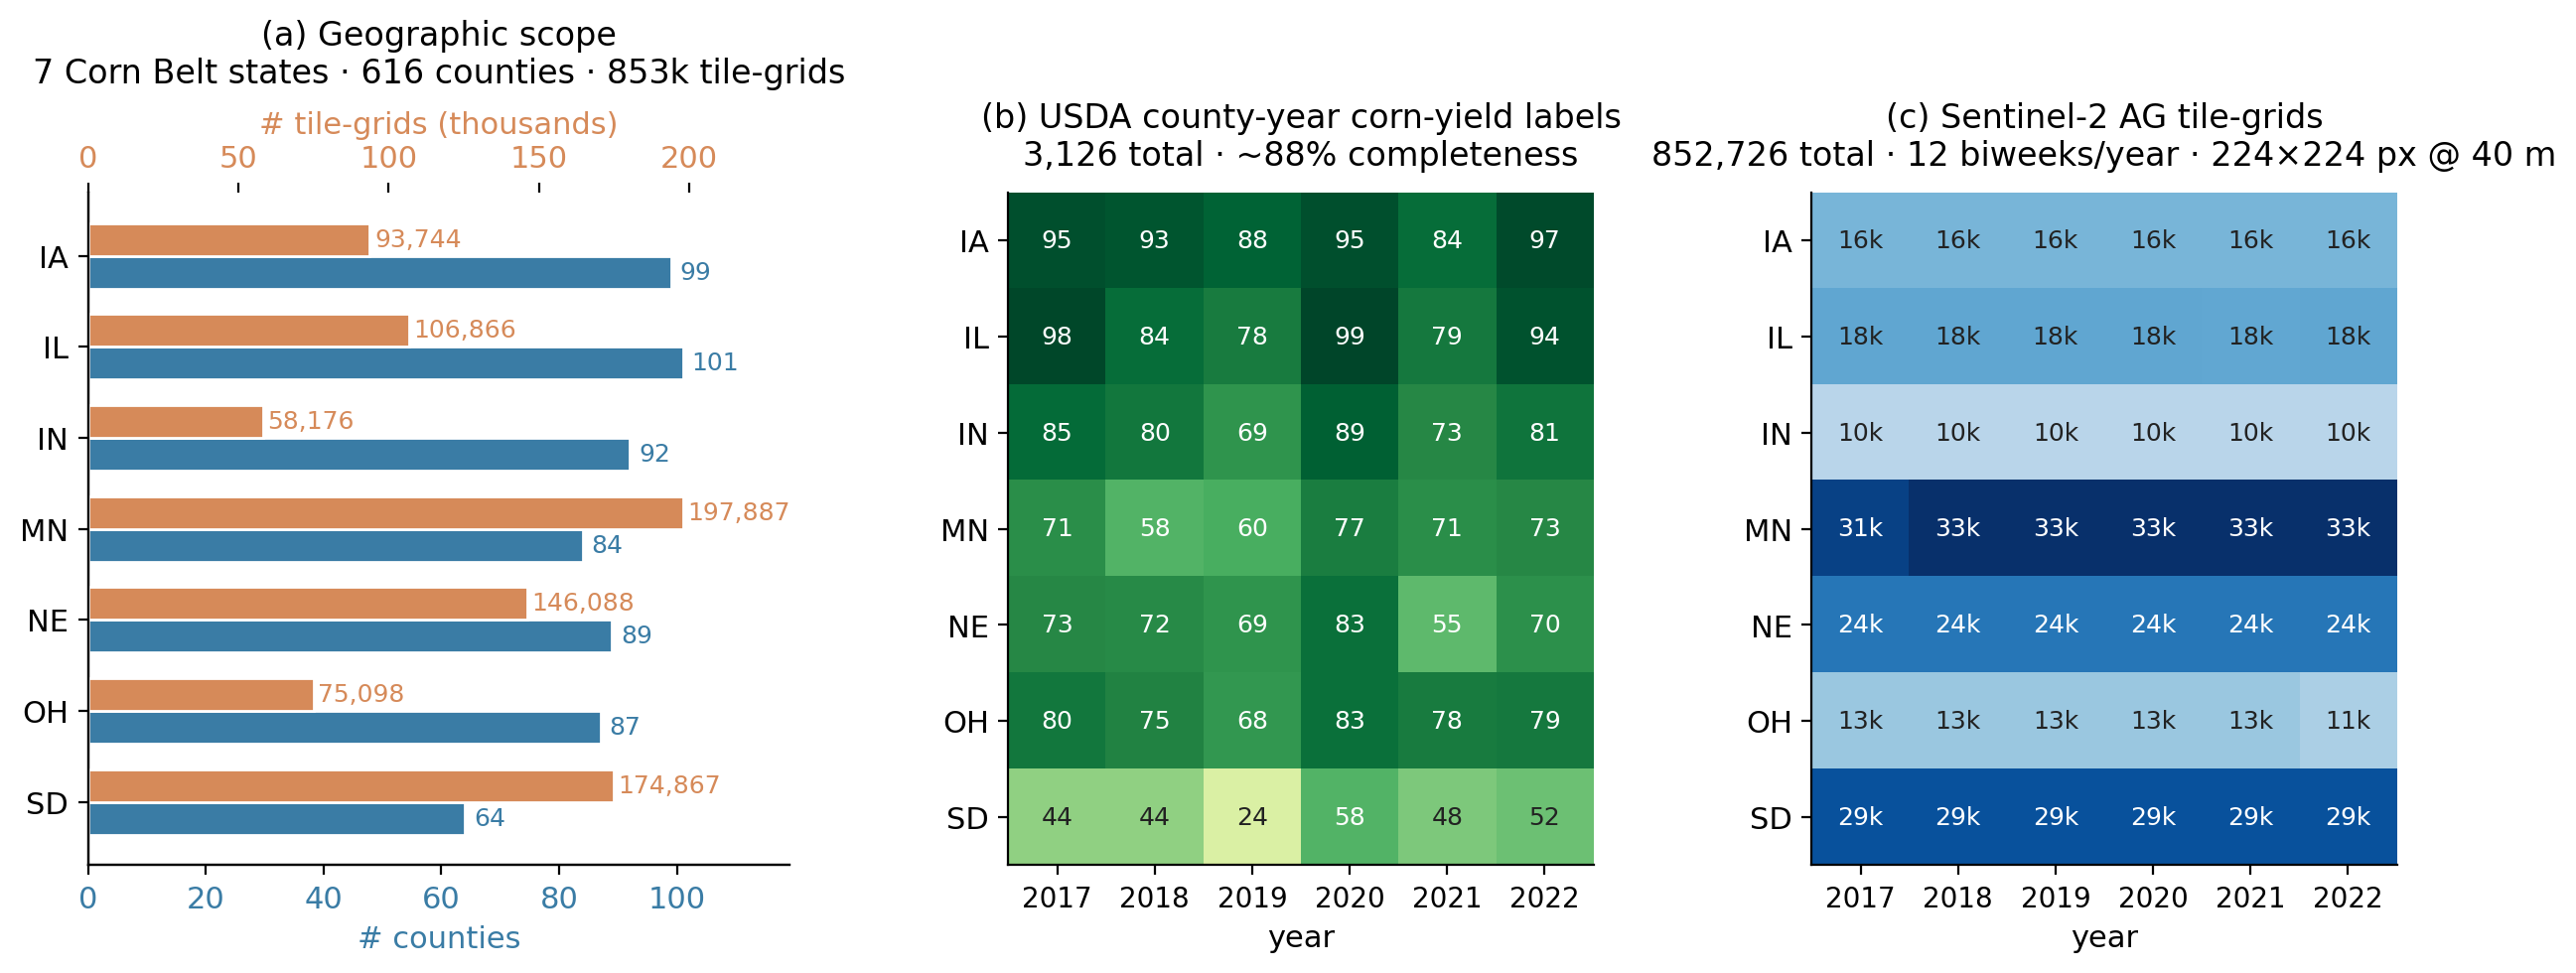
\includegraphics[width=\linewidth]{fig03_data_summary.png}
  \caption{Data scope. (a) Per-state county and tile-grid counts: 7 states,
  616 counties, 852{,}726 tile-grids in total. (b) USDA county-year corn-yield
  label counts (3{,}126 total, $\sim$88\,\% completeness; cells without labels
  are small low-acreage counties suppressed by USDA for privacy). (c)
  Sentinel-2 AG tile-grid counts per (state, year), 12 biweeks per year.}
  \label{fig:data-summary}
\end{figure}

\begin{figure}[H]
  \centering
  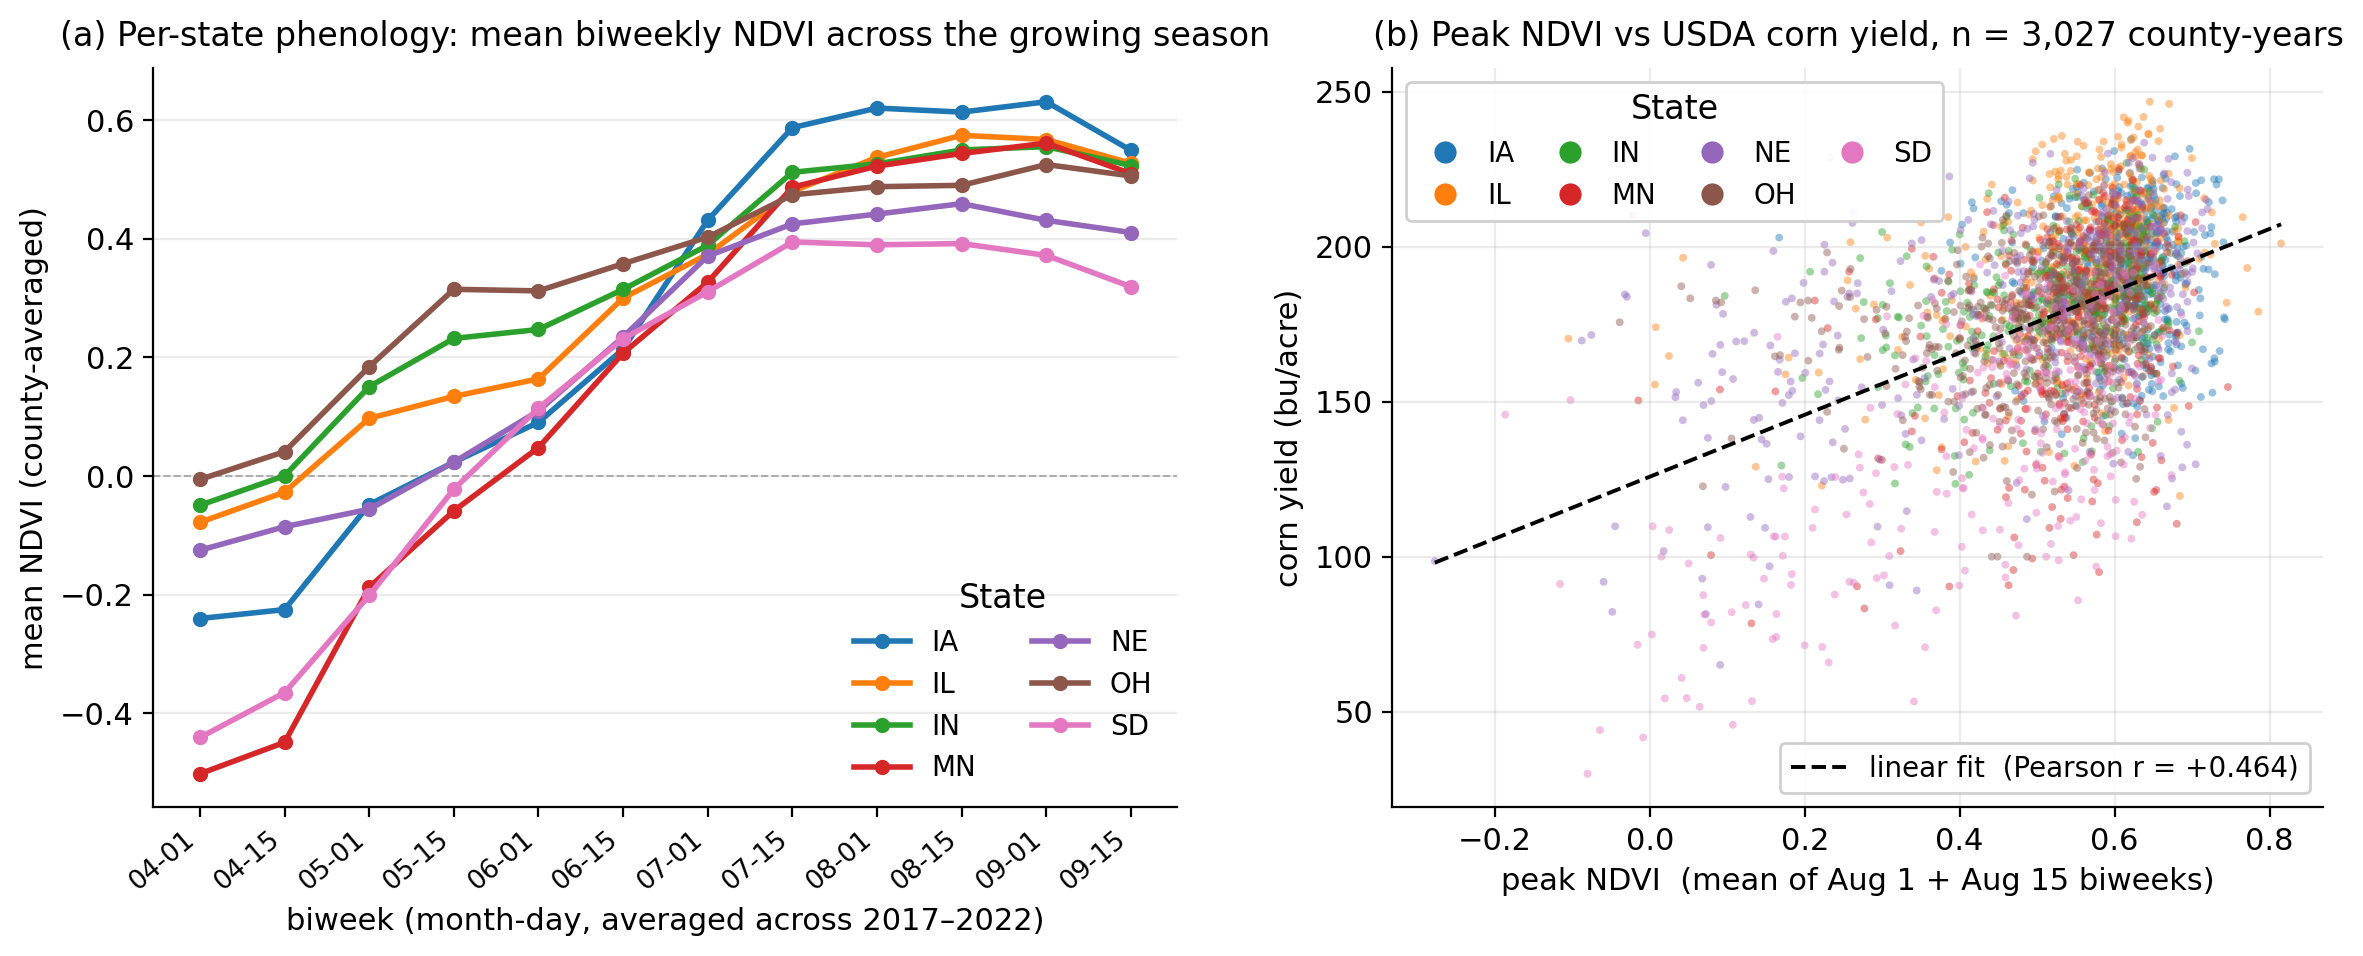
\includegraphics[width=\linewidth]{fig04_ndvi_phenology.png}
  \caption{Per-pixel NDVI computed from CropNet's quantised B04 + B08 reference
  channels. (a) Per-state mean biweekly NDVI across the growing season
  (averaged over 2017--2022); the canonical green-up $\to$ Aug peak $\to$
  senescence pattern is visible in all seven states, with MN/SD starting
  notably negative in early April due to lingering snow and wet bare soil.
  (b) Per-county-year peak NDVI (mean of Aug 1 + Aug 15 biweeks) vs.\ USDA
  corn yield, coloured by state, with the global linear fit and Pearson $r$
  overlaid. Within-state correlations are higher than the global $r=+0.46$.}
  \label{fig:ndvi-phen}
\end{figure}

\subsection{Full encoder $\times$ probe grid}

\begin{table}[H]
\centering
\caption{Full encoder $\times$ probe $\times$ split $\times$ \{with, without\} state+year features grid for the
four deep-learning encoders ($R^2$, higher is better). $\pm$SY denotes whether the 7-state one-hot and the
year scalar are appended to the encoder features before fitting the probe. Bold values are the per-column
winner; an asterisk ($^{*}$) marks our model. RMSE versions omitted for compactness.}
\label{tab:full-grid}
\small
\begin{tabular}{lcccccccc}
\toprule
 & \multicolumn{4}{c}{\textbf{Time split}} & \multicolumn{4}{c}{\textbf{County split}} \\
\cmidrule(lr){2-5}\cmidrule(lr){6-9}
 & \multicolumn{2}{c}{Ridge} & \multicolumn{2}{c}{LGBM} & \multicolumn{2}{c}{Ridge} & \multicolumn{2}{c}{LGBM} \\
\cmidrule(lr){2-3}\cmidrule(lr){4-5}\cmidrule(lr){6-7}\cmidrule(lr){8-9}
Encoder & $-$SY & $+$SY & $-$SY & $+$SY & $-$SY & $+$SY & $-$SY & $+$SY \\
\midrule
\textbf{Geo-SimCLR*} & \textbf{+0.669} & +0.548 & +0.624 & +0.542 & +0.451 & +0.452 & \textbf{+0.596} & \textbf{+0.660} \\
DINOv2-base & +0.661 & \textbf{+0.609} & \textbf{+0.641} & \textbf{+0.582} & \textbf{+0.541} & \textbf{+0.559} & +0.495 & +0.602 \\
Prithvi-EO 2.0 & +0.550 & +0.573 & +0.424 & +0.483 & +0.358 & +0.391 & +0.282 & +0.519 \\
Random ResNet-18 & +0.558 & +0.565 & +0.506 & +0.560 & +0.312 & +0.354 & +0.404 & +0.583 \\
\bottomrule
\end{tabular}
\end{table}


\subsection{Plain PHATE and UMAP corroboration of the collapse}

\begin{figure}[H]
  \centering
  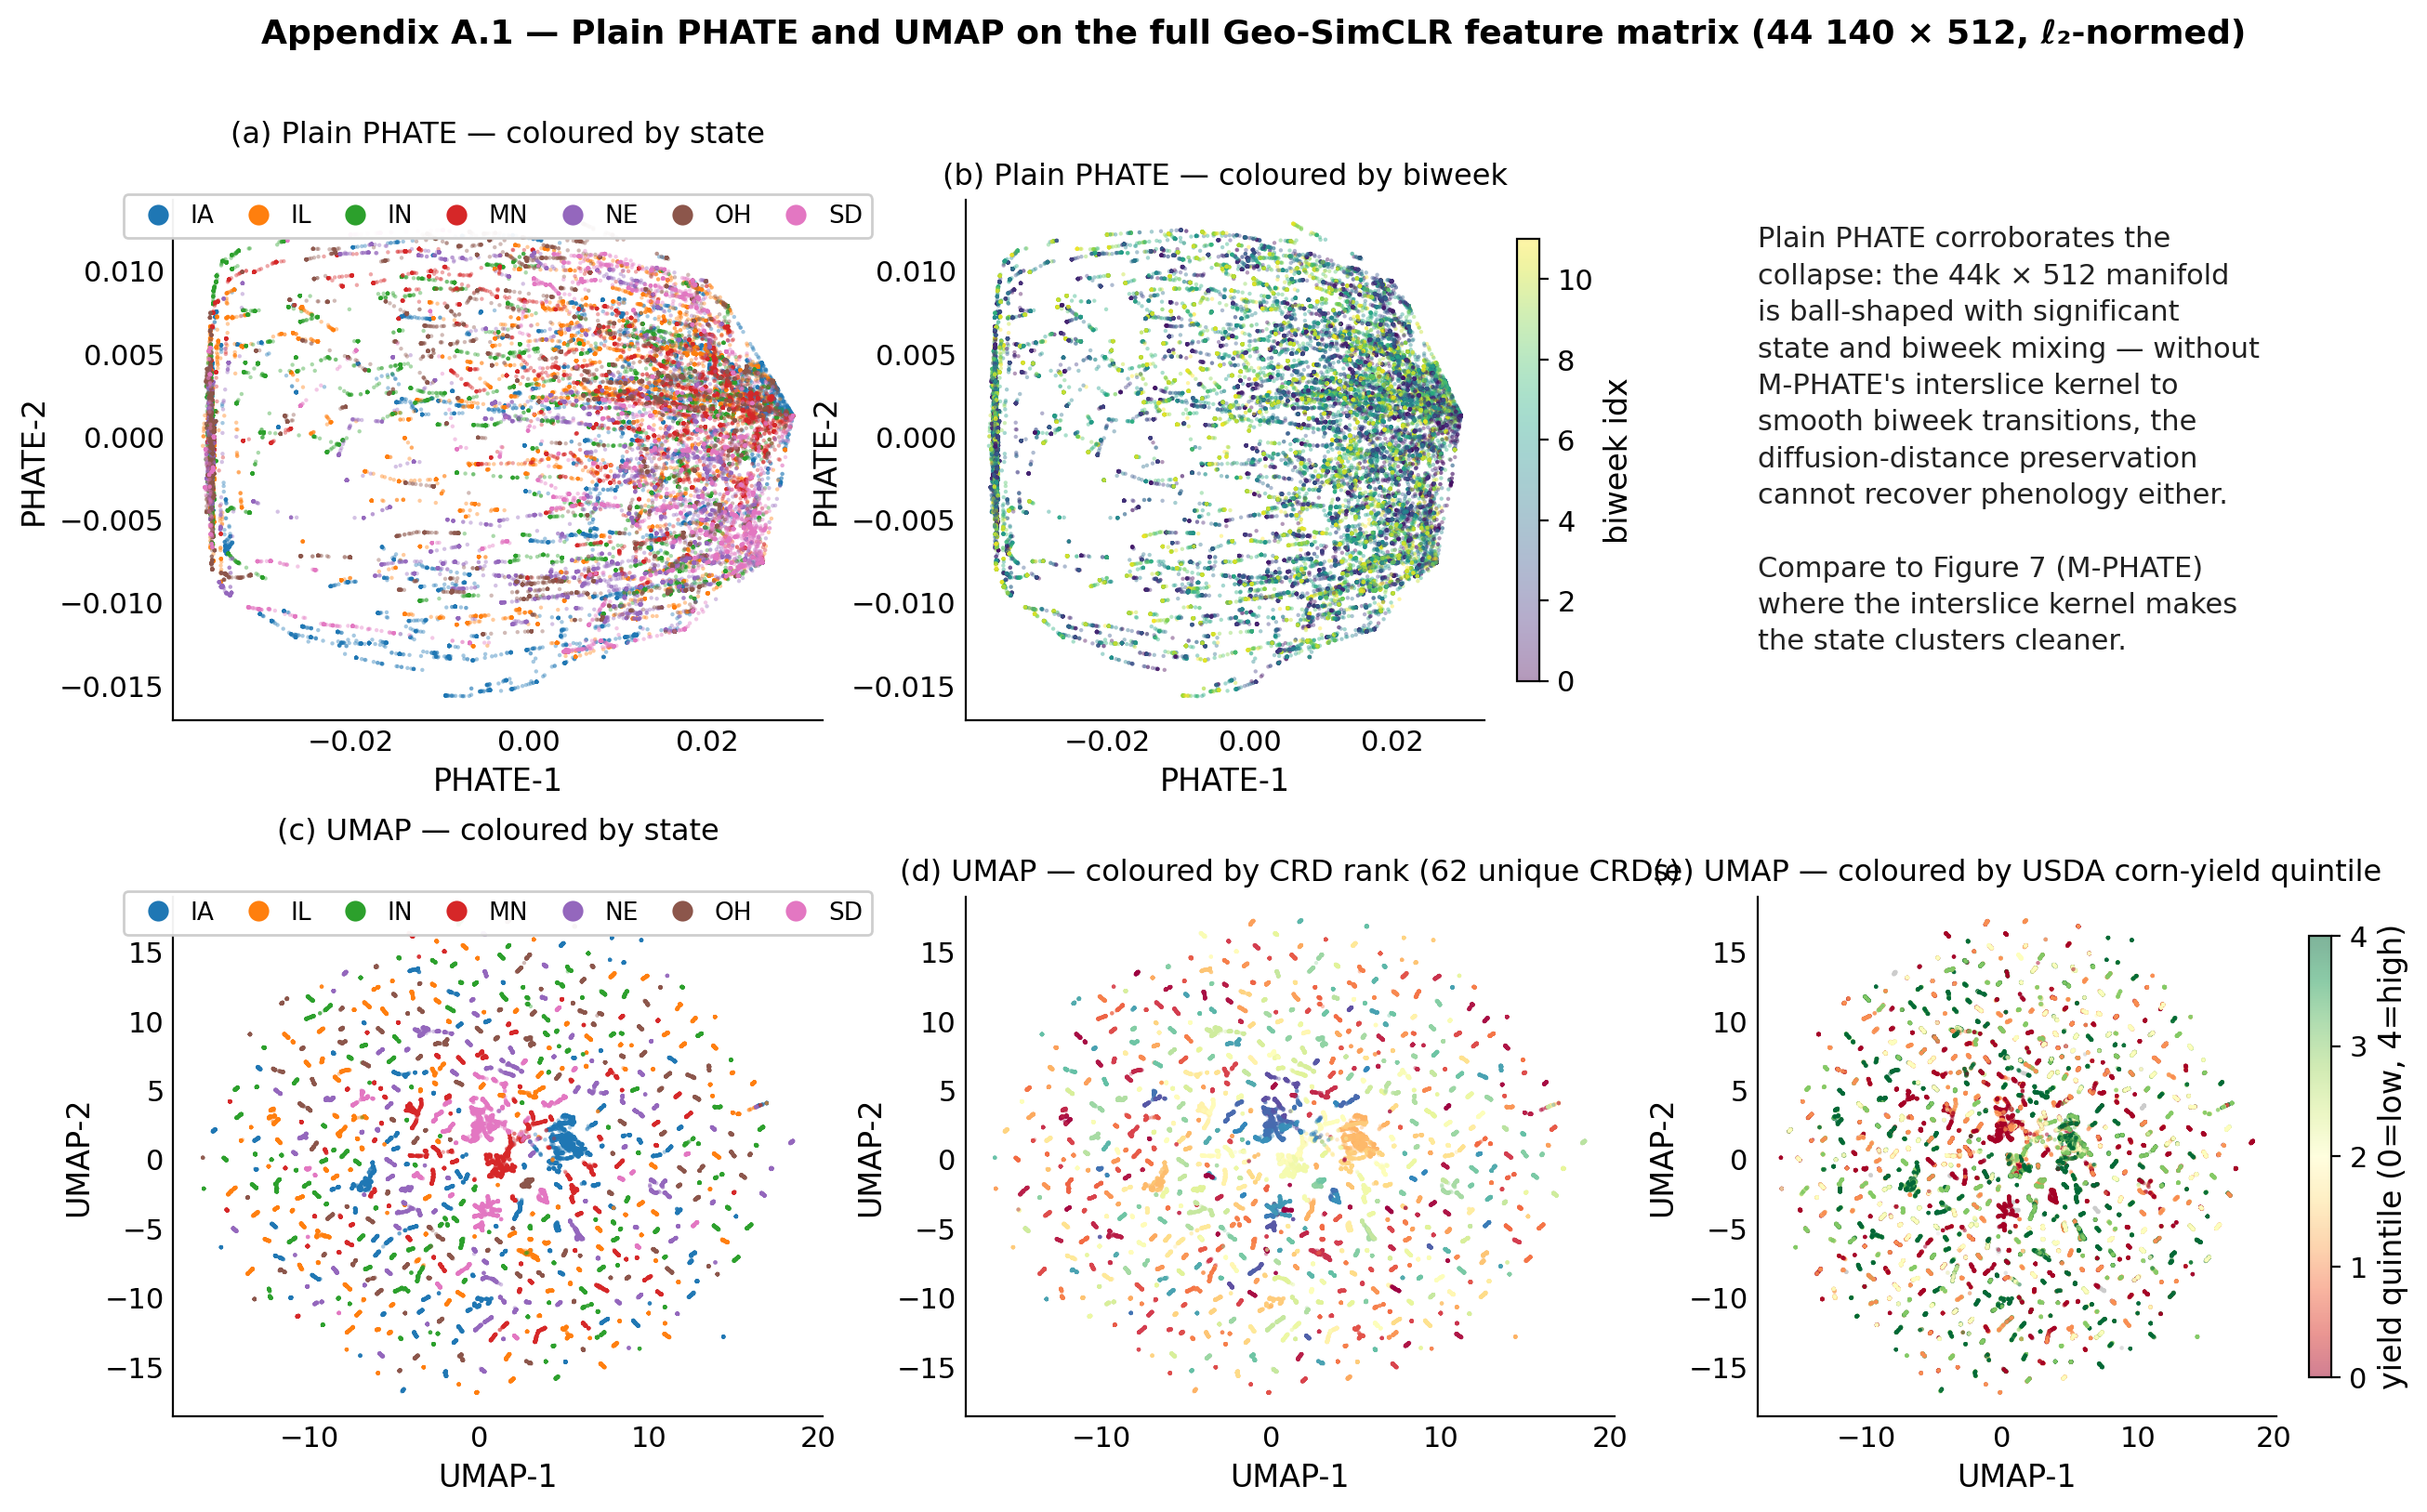
\includegraphics[width=\linewidth]{figA1_phate_umap.png}
  \caption{Plain PHATE \citep{moon2019phate} and UMAP \citep{mcinnes2018umap}
  on the same 44{,}140 $\times$ 512 $\ell_2$-normalised feature matrix used
  for the collapse diagnostic in Section~\ref{sec:results-collapse}. (a, b)
  PHATE coloured by state and biweek; without M-PHATE's inter-slice kernel,
  the diffusion-distance preservation cannot recover phenology either, and
  the embedding is ball-shaped with significant state and biweek mixing.
  (c, d, e) UMAP coloured by state, by Crop Reporting District rank
  (62 unique CRDs), and by USDA corn-yield quintile. All three views
  corroborate the SVD-based collapse evidence: the manifold is too dense for
  UMAP's local-distance focus to find clean state boundaries.}
  \label{fig:phate-umap}
\end{figure}

\subsection{Full hyperparameter table}

\begin{table}[H]
\centering
\caption{Full hyperparameter and training-protocol summary for Geo-SimCLR self-supervised pre-training,
the supervised end-to-end ConvLSTM baseline, and the frozen-feature probe protocol. Values are exactly
those used to produce the headline results in Table~\ref{tab:headline}.}
\label{tab:hyperparameters}
\small
\begin{tabular}{p{5.5cm}p{8.5cm}}
\toprule
\multicolumn{2}{l}{\textbf{Geo-SimCLR self-supervised pre-training (notebook 04)}} \\
\midrule
Backbone & ResNet-18 from scratch (3-channel input, no adapter) \\
Projection head & MLP $512 \to 256 \to 128$ with BN+ReLU; $\ell_2$-normalized output \\
Total parameters & $11.34\,\mathrm{M}$ (encoder $11.18\,\mathrm{M}$ + projector $0.16\,\mathrm{M}$) \\
Loss & NT-Xent on $\ell_2$-normalized 128-d projections \\
Temperature $\tau$ & 0.20 \\
Batch size & 1024 (effective; DataParallel across 2 GPUs) \\
Optimizer & AdamW, $\mathrm{lr}=10^{-3}$, $\mathrm{wd}=10^{-4}$ \\
Scheduler & LinearLR warmup ($\mathrm{lr}/100 \to \mathrm{lr}$) over 5 epochs, then CosineAnnealingLR ($\eta_\mathrm{min}=10^{-6}$) for 45 epochs \\
Epochs & 50 \\
Mixed precision & AMP (bfloat16 autocast) + GradScaler \\
Anchors per epoch & $\sim 644{,}922$ after dropping NaN-CRD anchors \\
CRD-balanced sampling & WeightedRandomSampler, weights $\propto 1/(\#\mathrm{anchors\ per\ CRD})$, 61 CRDs \\
Augmentations (per view) & hflip 0.5; vflip 0.5; rot90 $k\!\in\!\{1,2,3\}$ p=0.75; random crop 160--208 px $\to$ resize 224; sharpness $\times 2.0$ p=0.5; per-band intensity $\times U[0.8,1.2]$ p=0.8; per-band Gaussian noise $\sigma=0.02$; per-band z-score \\
Excluded augmentations & spectral band dropout, RGB color jitter, mixup \\
Data scope & 7 states (IA, IL, IN, MN, NE, OH, SD), 6 years (2017--2022), Apr--Sep biweekly, 224$\times$224 px AG (B02, B08, B11) tiles \\
Wall time & $\sim$5--7 min / epoch $\times$ 50 ep $\approx$ 5\,h on 2 GPUs \\
\midrule
\multicolumn{2}{l}{\textbf{ConvLSTM end-to-end supervised baseline (notebook 05)}} \\
\midrule
Per-frame encoder & ResNet-18 (random init) producing 512-d per biweek \\
Recurrence & single-layer LSTM, hidden 256 \\
Head & MLP $256 \to 64 \to 1$, dropout 0.2 \\
Target & $z$-scored on training yields \\
Optimizer & AdamW, $\mathrm{lr}=10^{-4}$, $\mathrm{wd}=10^{-4}$ \\
Scheduler & CosineAnnealingLR ($T_\mathrm{max}=30$, $\eta_\mathrm{min}=10^{-6}$) \\
Batch size / Epochs & 32 / 30; checkpoint = best 2021-validation RMSE \\
Augmentations & identical hflip / vflip / rot90 / random crop applied to all 12 biweek frames per example \\
\midrule
\multicolumn{2}{l}{\textbf{Frozen-feature probe protocol (notebook 05, all encoders)}} \\
\midrule
Pooling & mean-pool tile features per (fips, year, biweek), then per (fips, year) \\
Linear probe & Ridge, $\alpha\!=\!1$ (no CV), no normalization \\
Tree probe & LightGBM: 300 trees, lr 0.05, num\_leaves 31, min\_child\_samples 5 \\
LGBM early stopping & 20 rounds on 2021 validation set (time split only) \\
State+year features & 7-state one-hot + year scalar appended when applicable \\
Splits & \textit{Time}: train 2017--2020 / val 2021 / test 2022. \textit{County}: random 20\% FIPS held out, all years. \\
Bootstrap CIs & $n=200$ paired resamples of held-out predictions, percentiles 2.5/97.5 \\
\bottomrule
\end{tabular}
\end{table}


\subsection{Compute footprint}
Total wall time for the headline pipeline (data acquisition, baselines,
self-supervised pre-training, feature extraction, downstream probes, and
visualisation) was approximately 14 hours on a Yale High-Performance Computing
node with 18 CPU cores, 24 GiB of RAM, and 2 GPUs. Self-supervised
pre-training itself was the dominant cost at $\sim$19 hours
(50 epochs $\times$ $\sim$12 minutes/epoch with AMP and DataParallel across
2 GPUs). Feature extraction for the four encoders took $\sim$2 hours; probe
fitting and visualisation ran in $\sim$1 hour total on a local CPU.

\end{document}
